\documentclass[8pt,aspectratio=1610]{beamer}
\usepackage[utf8]{inputenc}
\usepackage{booktabs}
\usepackage{array}
\usepackage{graphicx}
\usepackage{xcolor}
\usepackage{tikz}
\usetikzlibrary{positioning,arrows.meta,decorations.pathreplacing,calc,shadows}
\usepackage{pgfplots}
\pgfplotsset{compat=1.18}
\usepackage{amsmath}
\usepackage{amssymb}
\usepackage{amsfonts}
\usepackage{algorithm}
\usepackage{algorithmic}

\usetheme{metropolis}
\usecolortheme{wolverine}
\metroset{progressbar=frametitle,block=fill}
\setbeamertemplate{navigation symbols}{}

% Define custom colors complementing the Wolverine theme
\definecolor{maizelight}{RGB}{255, 203, 5}
\definecolor{maizedark}{RGB}{255, 167, 0}
\definecolor{bluelight}{RGB}{0, 39, 76}
\definecolor{tealaccent}{RGB}{0, 128, 128}
\definecolor{orangeaccent}{RGB}{255, 138, 51}

% Customize block colors
\setbeamercolor{block title}{bg=bluelight,fg=white}
\setbeamercolor{block body}{bg=bluelight!10,fg=black}

\setbeamercolor{block title example}{bg=maizelight,fg=black}
\setbeamercolor{block body example}{bg=maizelight!15,fg=black}

\setbeamercolor{block title alerted}{bg=orangeaccent,fg=white}
\setbeamercolor{block body alerted}{bg=orangeaccent!15,fg=black}

\newenvironment<>{techblock}[1]{%
  \setbeamercolor{block title}{bg=tealaccent,fg=white}%
  \setbeamercolor{block body}{bg=tealaccent!10,fg=black}%
  \begin{block}#2{#1}}{\end{block}}

\newenvironment<>{tipblock}[1]{%
  \setbeamercolor{block title}{bg=maizedark,fg=black}%
  \setbeamercolor{block body}{bg=maizedark!15,fg=black}%
  \begin{block}#2{#1}}{\end{block}}

\title{Model Selection and Evaluation}
\subtitle{CMSC 173 - Machine Learning}
\author{Course Lecture}
\date{}

\begin{document}

\begin{frame}
\titlepage
\end{frame}

\begin{frame}{Outline}
\tableofcontents
\end{frame}

% ========================================
% Section: Introduction
% ========================================

\section{Introduction to Model Selection}

\begin{frame}{The Model Selection Problem}
\centering
\textbf{Central Question: How do we choose the best model?}

\vspace{0.3cm}

\begin{columns}[t]
\begin{column}{0.48\textwidth}
\begin{alertblock}{Challenges}
\begin{itemize}
\setlength{\itemsep}{2pt}
\item Multiple algorithms available
\item Different hyperparameters
\item Trade-offs between complexity and performance
\item Avoiding overfitting
\item Generalization to unseen data
\end{itemize}
\end{alertblock}
\end{column}

\begin{column}{0.48\textwidth}
\begin{exampleblock}{Goals}
\begin{itemize}
\setlength{\itemsep}{2pt}
\item Select optimal model architecture
\item Tune hyperparameters effectively
\item Ensure reliable performance
\item Balance bias and variance
\item Maximize generalization
\end{itemize}
\end{exampleblock}
\end{column}
\end{columns}

\vspace{0.2cm}

\begin{techblock}{Key Insight}
Model selection is not just about training performance, but about how well the model generalizes to new, unseen data.
\end{techblock}
\end{frame}

\begin{frame}{Model Selection Pipeline}
\begin{center}
\begin{tikzpicture}[node distance=1.5cm, every node/.style={font=\small}]
\node[rectangle, draw, fill=blue!20, minimum width=2.5cm, minimum height=0.8cm] (data) {Data};
\node[rectangle, draw, fill=green!20, minimum width=2.5cm, minimum height=0.8cm, right=of data] (split) {Train/Val/Test Split};
\node[rectangle, draw, fill=yellow!20, minimum width=2.5cm, minimum height=0.8cm, right=of split] (train) {Train Models};
\node[rectangle, draw, fill=orange!20, minimum width=2.5cm, minimum height=0.8cm, below=0.8cm of train] (validate) {Validate \& Select};
\node[rectangle, draw, fill=purple!20, minimum width=2.5cm, minimum height=0.8cm, left=of validate] (test) {Test Final Model};

\draw[->, thick] (data) -- (split);
\draw[->, thick] (split) -- (train);
\draw[->, thick] (train) -- (validate);
\draw[->, thick] (validate) -- (test);
\end{tikzpicture}
\end{center}

\vspace{0.2cm}

\begin{itemize}
\item \textbf{Split:} Divide data into training, validation, and test sets
\item \textbf{Train:} Fit multiple candidate models
\item \textbf{Validate:} Compare models on validation set
\item \textbf{Select:} Choose best performing model
\item \textbf{Test:} Final evaluation on held-out test set
\end{itemize}
\end{frame}

\begin{frame}{Train-Validation-Test Split}
\begin{center}
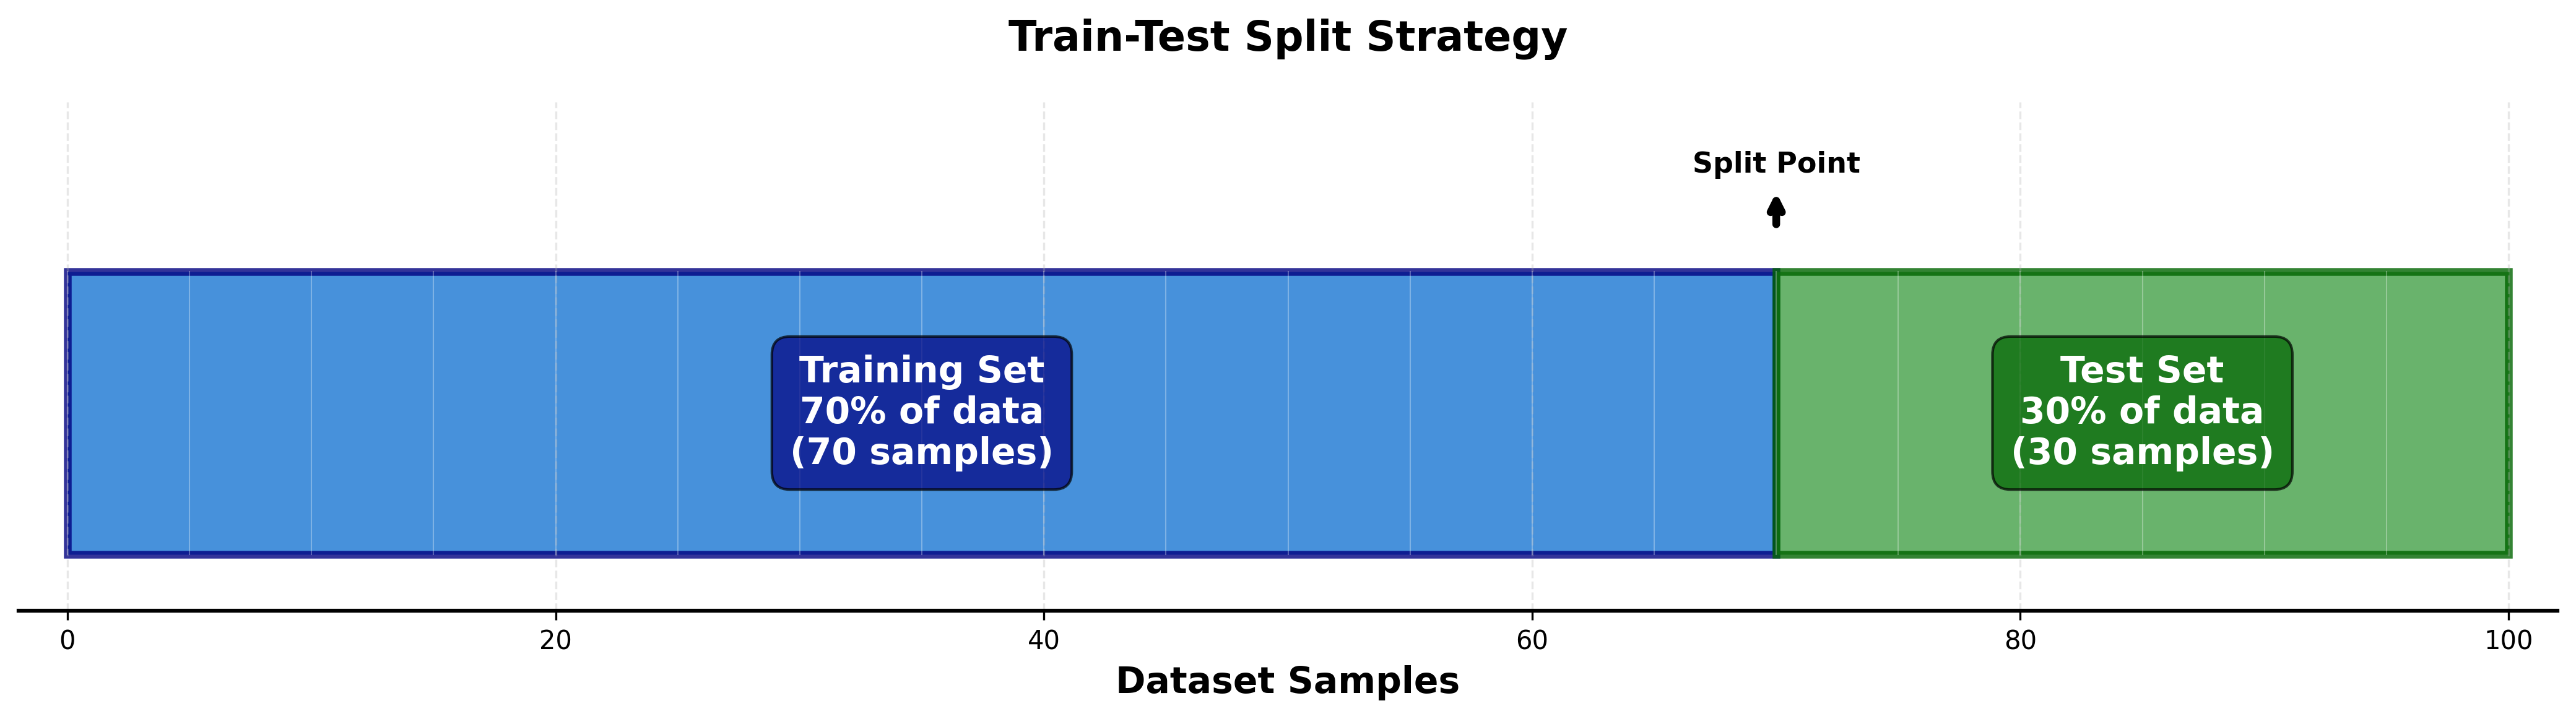
\includegraphics[width=0.85\textwidth]{../figures/train_test_split.png}
\end{center}

\vspace{0.1cm}

\begin{columns}[t]
\begin{column}{0.32\textwidth}
\begin{block}{Training Set}
\begin{itemize}
\setlength{\itemsep}{1pt}
\item Model fitting
\item Learning parameters
\item 60-70\% of data
\end{itemize}
\end{block}
\end{column}

\begin{column}{0.32\textwidth}
\begin{block}{Validation Set}
\begin{itemize}
\setlength{\itemsep}{1pt}
\item Model selection
\item Hyperparameter tuning
\item 15-20\% of data
\end{itemize}
\end{block}
\end{column}

\begin{column}{0.32\textwidth}
\begin{block}{Test Set}
\begin{itemize}
\setlength{\itemsep}{1pt}
\item Final evaluation
\item Unbiased estimate
\item 15-20\% of data
\end{itemize}
\end{block}
\end{column}
\end{columns}
\end{frame}

% ========================================
% Section: Bias-Variance Decomposition
% ========================================

\section{Bias-Variance Decomposition}

\begin{frame}{Understanding Prediction Error}
For a regression problem, the expected prediction error can be decomposed:

\vspace{0.2cm}

\begin{alertblock}{Error Decomposition}
\begin{equation*}
\mathbb{E}[(y - \hat{f}(x))^2] = \text{Bias}^2[\hat{f}(x)] + \text{Var}[\hat{f}(x)] + \sigma^2
\end{equation*}
\end{alertblock}

\vspace{0.2cm}

\begin{columns}[t]
\begin{column}{0.32\textwidth}
\begin{block}{Bias}
\vspace{-0.1cm}
\begin{equation*}
\text{Bias}[\hat{f}] = \mathbb{E}[\hat{f}] - f
\end{equation*}
Error from wrong assumptions in the learning algorithm
\end{block}
\end{column}

\begin{column}{0.32\textwidth}
\begin{block}{Variance}
\vspace{-0.1cm}
\begin{equation*}
\text{Var}[\hat{f}] = \mathbb{E}[(\hat{f} - \mathbb{E}[\hat{f}])^2]
\end{equation*}
Error from sensitivity to training set variations
\end{block}
\end{column}

\begin{column}{0.32\textwidth}
\begin{block}{Irreducible Error}
\vspace{-0.1cm}
\begin{equation*}
\sigma^2 = \text{Var}[\epsilon]
\end{equation*}
Noise in the data that cannot be reduced
\end{block}
\end{column}
\end{columns}
\end{frame}

\begin{frame}{The Bias-Variance Tradeoff}
\begin{center}
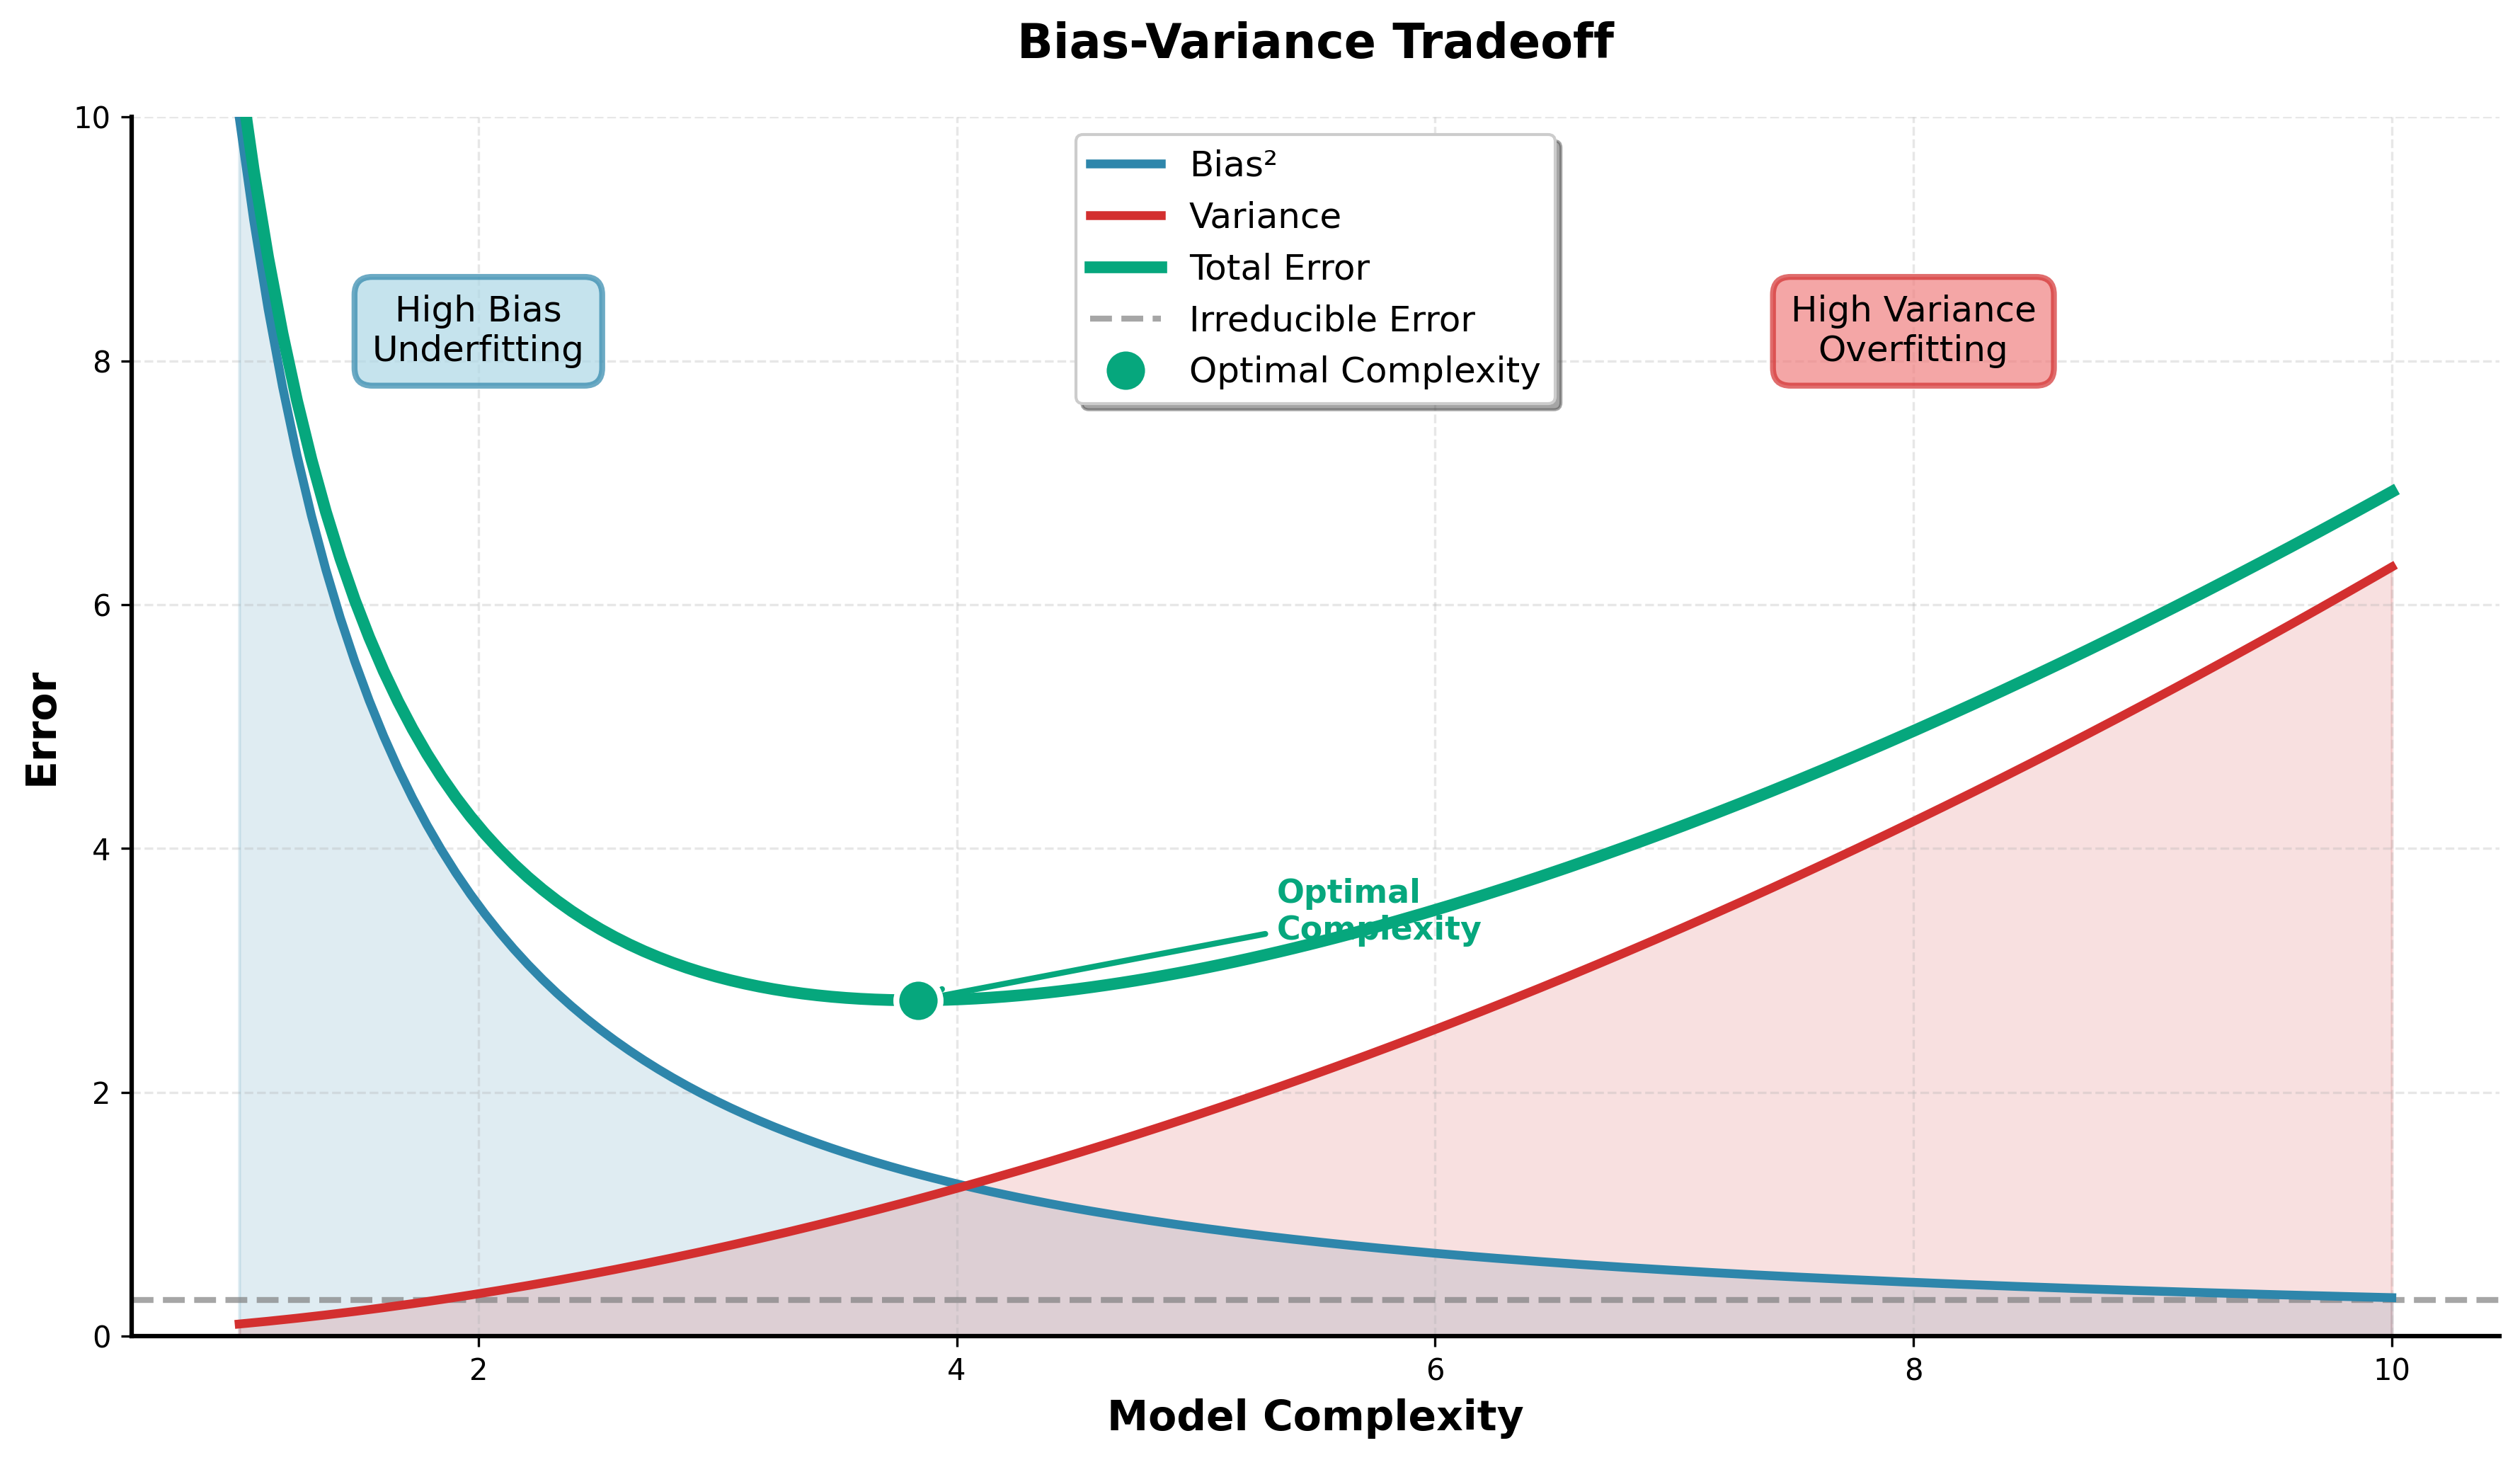
\includegraphics[width=0.75\textwidth]{../figures/bias_variance_tradeoff.png}
\end{center}

\vspace{0.1cm}

\begin{tipblock}{Key Insight}
\begin{itemize}
\setlength{\itemsep}{2pt}
\item As model complexity increases, bias decreases but variance increases
\item The optimal model minimizes the total error (bias$^2$ + variance)
\item There exists a sweet spot that balances both sources of error
\end{itemize}
\end{tipblock}
\end{frame}

\begin{frame}{High Bias vs High Variance}
\begin{columns}[t]
\begin{column}{0.48\textwidth}
\begin{alertblock}{High Bias (Underfitting)}
\textbf{Characteristics:}
\begin{itemize}
\setlength{\itemsep}{1pt}
\item Overly simple model
\item Poor training performance
\item Poor test performance
\item Cannot capture data patterns
\end{itemize}

\vspace{0.1cm}
\textbf{Solutions:}
\begin{itemize}
\setlength{\itemsep}{1pt}
\item Increase model complexity
\item Add more features
\item Reduce regularization
\item Train longer
\end{itemize}
\end{alertblock}
\end{column}

\begin{column}{0.48\textwidth}
\begin{alertblock}{High Variance (Overfitting)}
\textbf{Characteristics:}
\begin{itemize}
\setlength{\itemsep}{1pt}
\item Overly complex model
\item Excellent training performance
\item Poor test performance
\item Memorizes training data
\end{itemize}

\vspace{0.1cm}
\textbf{Solutions:}
\begin{itemize}
\setlength{\itemsep}{1pt}
\item Simplify model
\item Get more training data
\item Increase regularization
\item Use early stopping
\end{itemize}
\end{alertblock}
\end{column}
\end{columns}
\end{frame}

\begin{frame}{Visualizing Underfitting and Overfitting}
\begin{center}
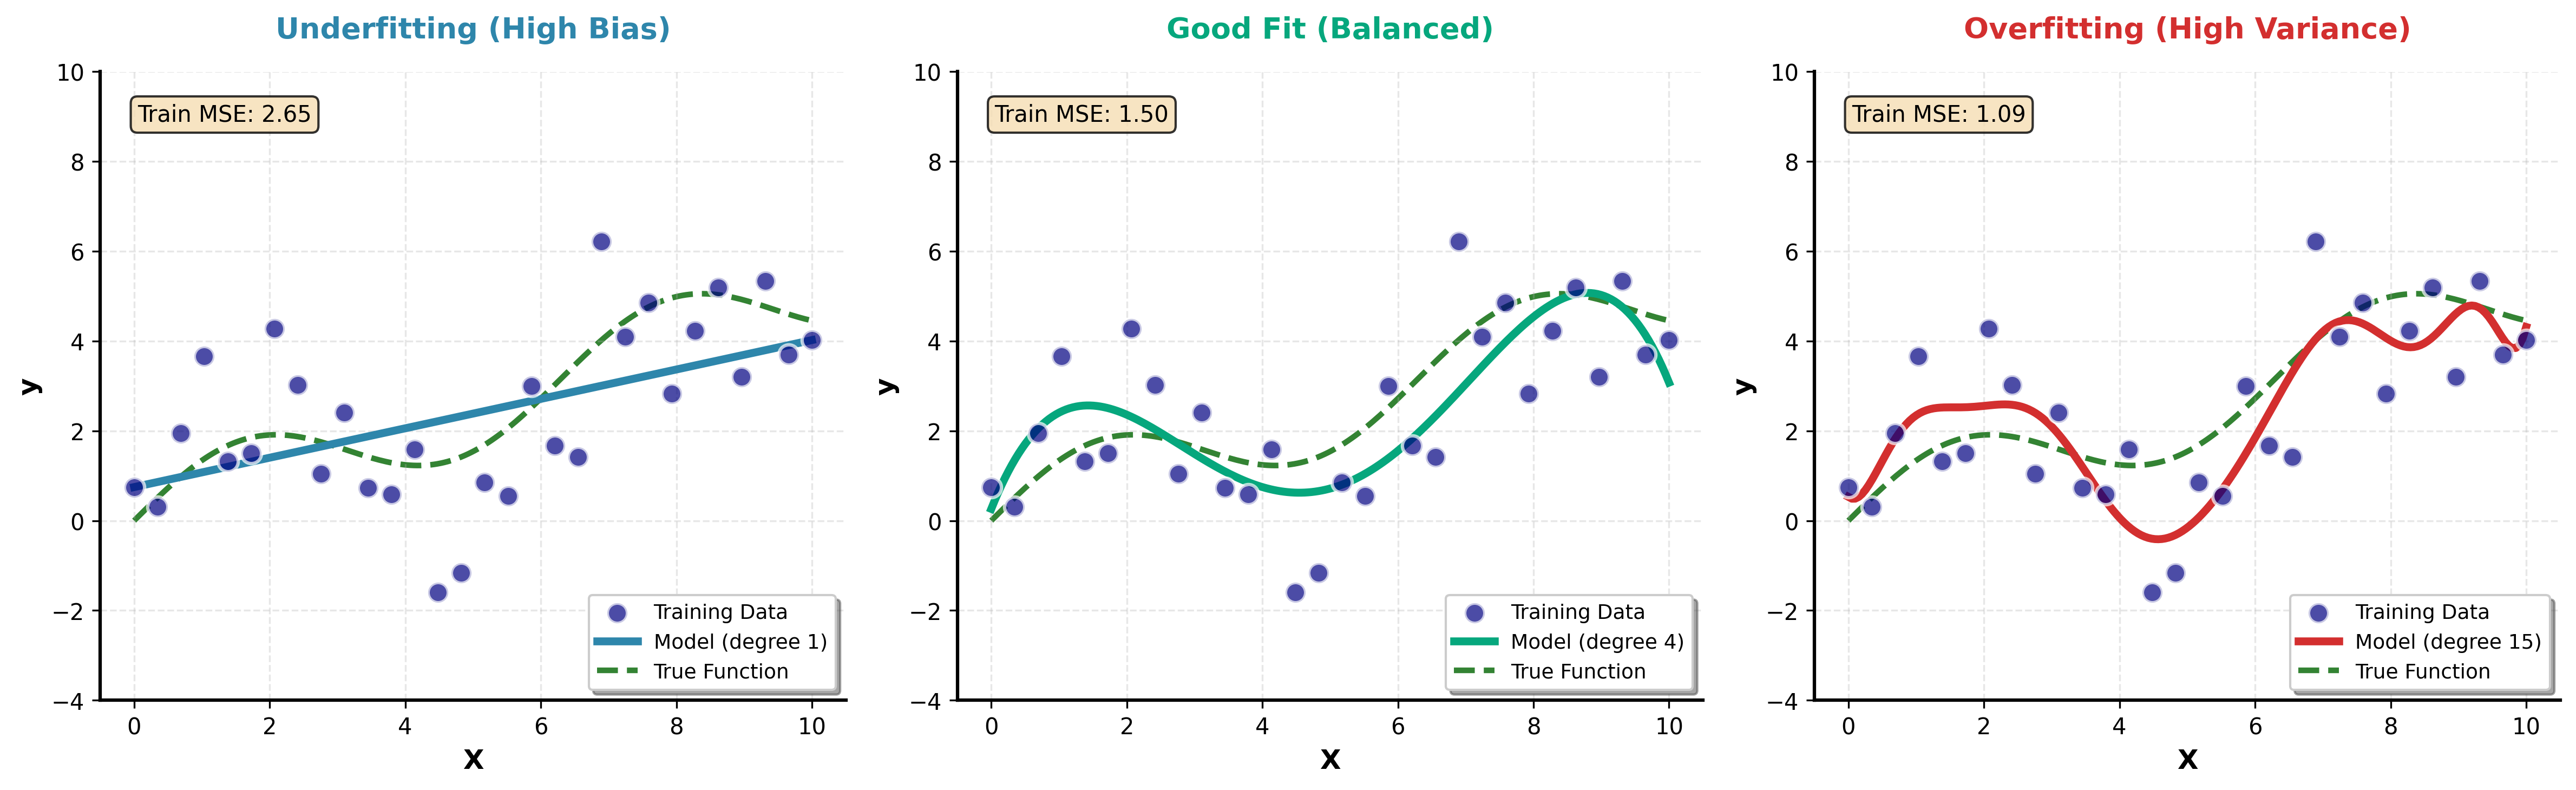
\includegraphics[width=0.95\textwidth]{../figures/underfitting_overfitting.png}
\end{center}

\vspace{0.1cm}

\begin{itemize}
\item \textbf{Left:} Underfitting - linear model cannot capture nonlinear relationship
\item \textbf{Center:} Good fit - balanced complexity captures true pattern
\item \textbf{Right:} Overfitting - high-degree polynomial fits noise
\end{itemize}
\end{frame}

\begin{frame}{Model Complexity and Error}
\begin{center}
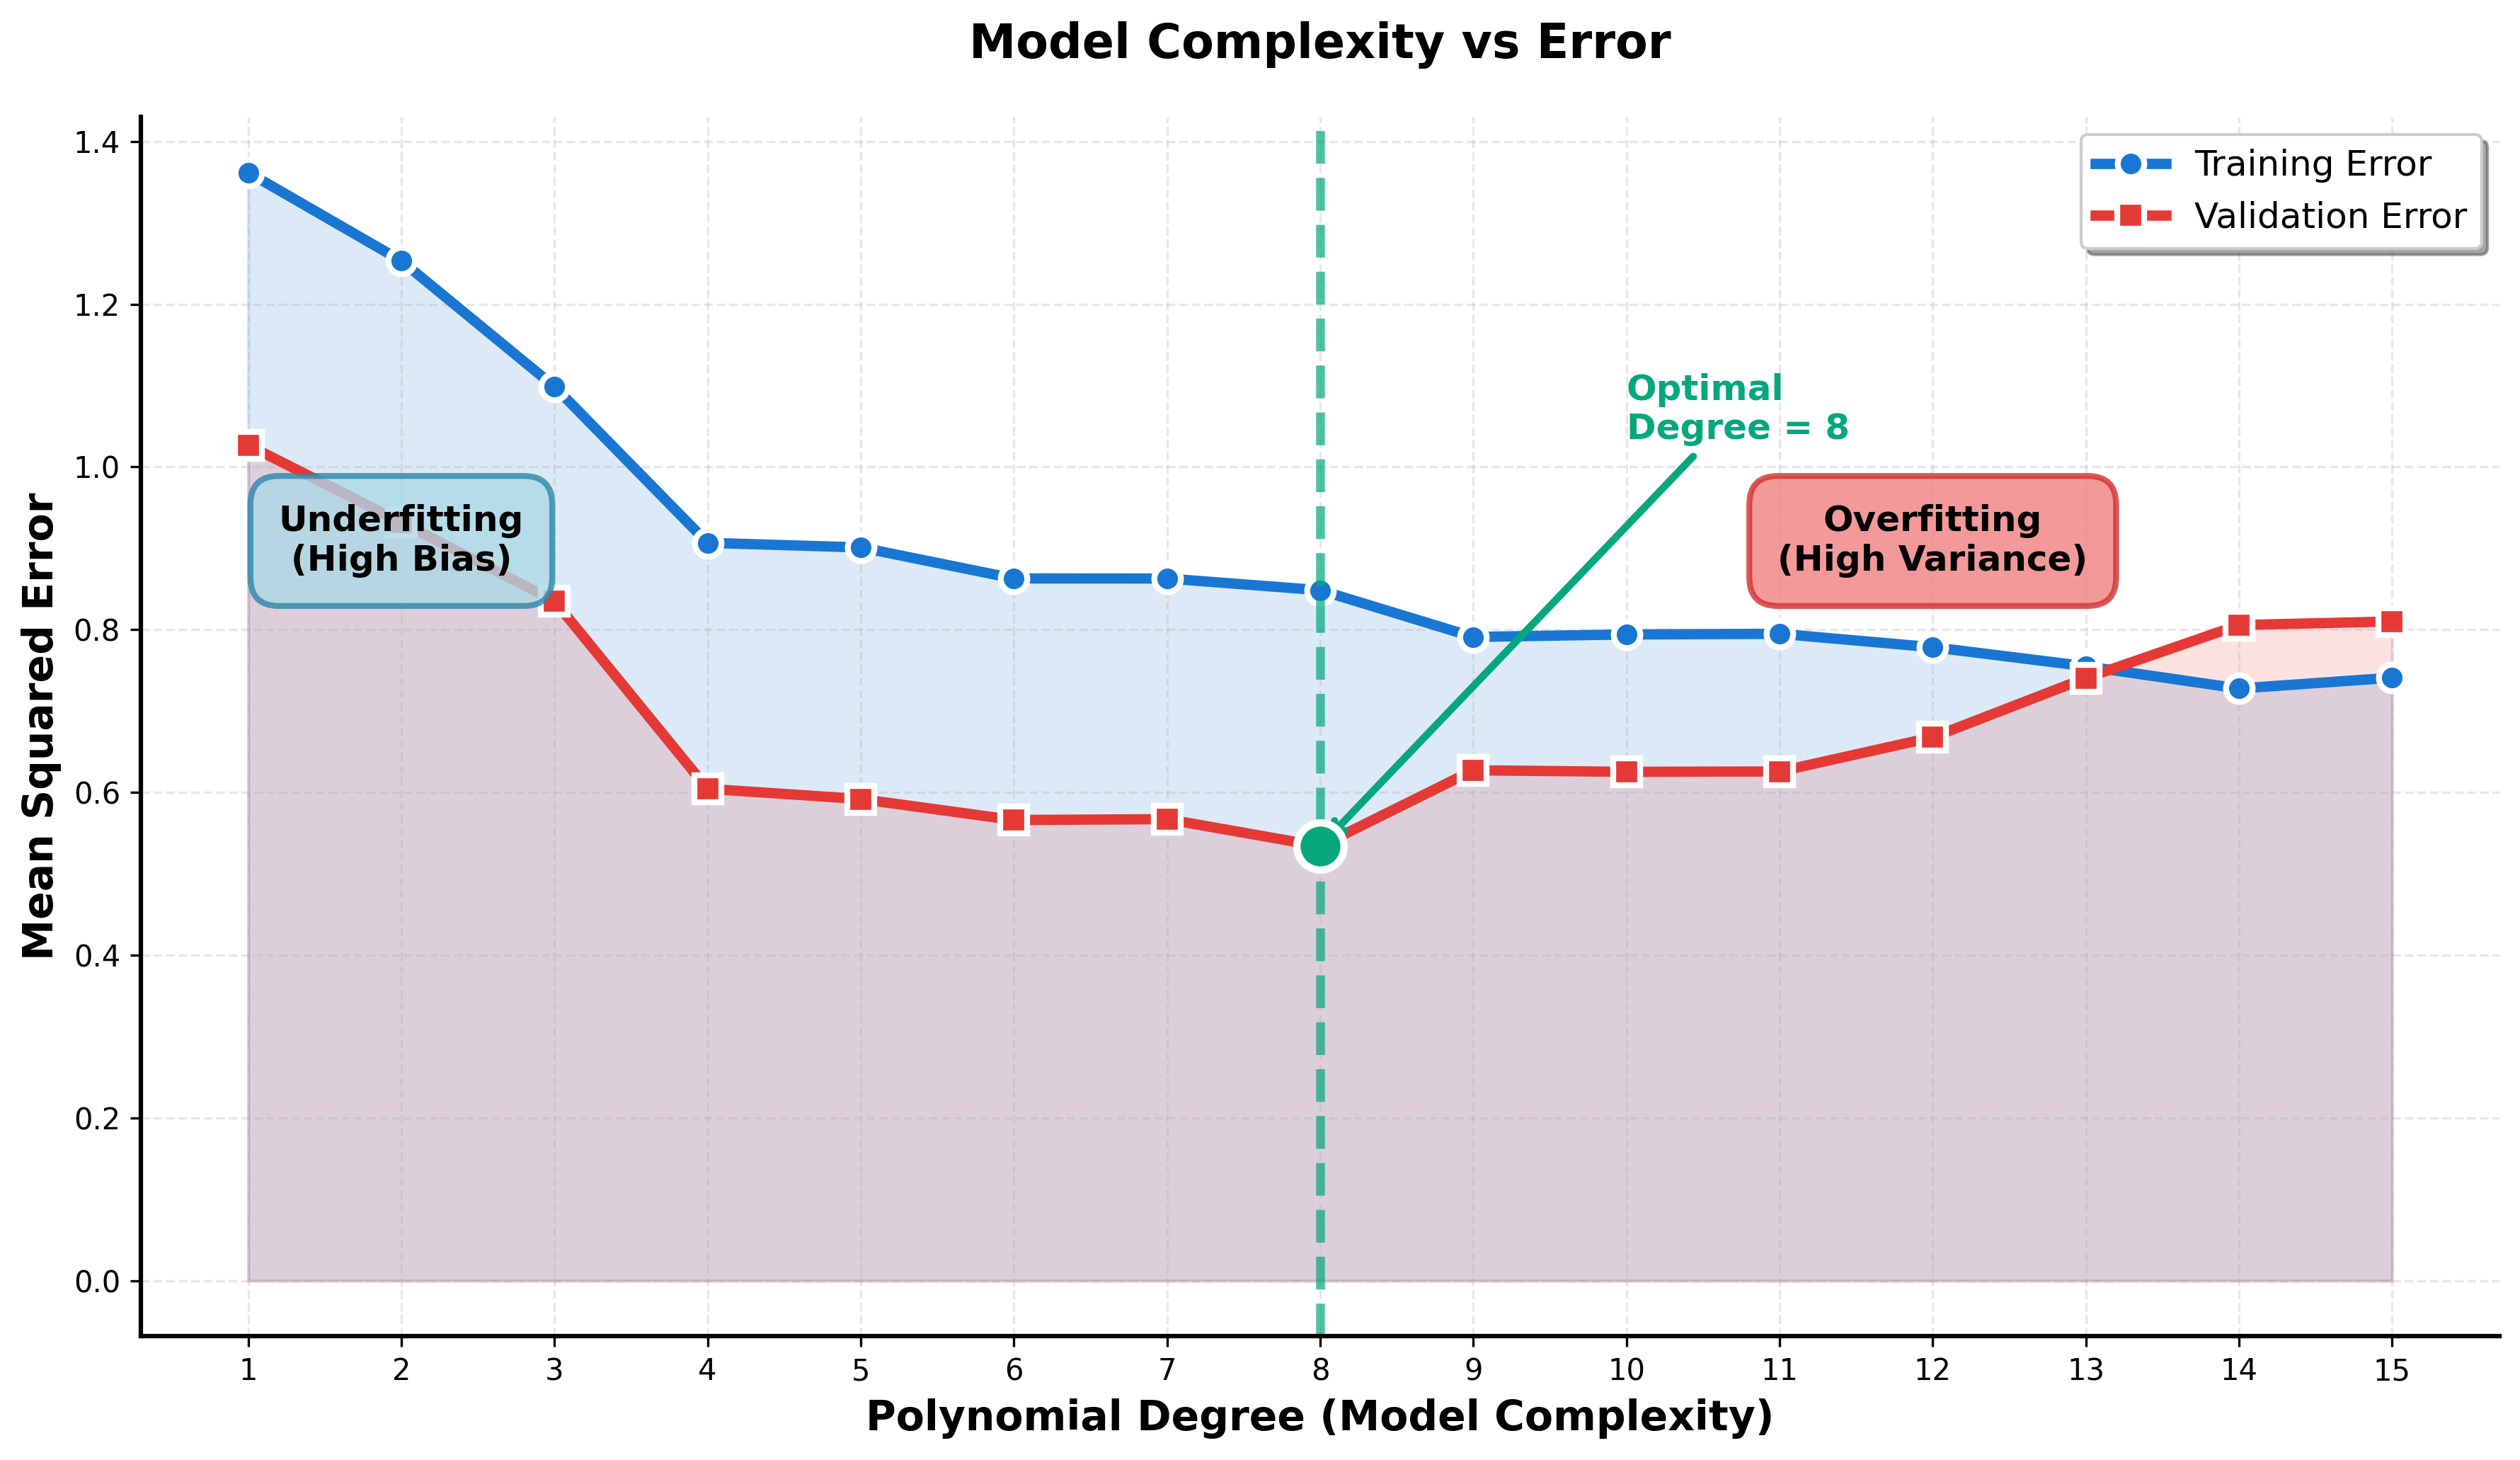
\includegraphics[width=0.8\textwidth]{../figures/model_complexity_curve.png}
\end{center}

\vspace{0.1cm}

\begin{techblock}{Observations}
\begin{itemize}
\setlength{\itemsep}{2pt}
\item Training error decreases monotonically with complexity
\item Validation error has a U-shaped curve
\item Gap between curves indicates overfitting
\item Optimal complexity minimizes validation error
\end{itemize}
\end{techblock}
\end{frame}

% ========================================
% Section: Model Validation and Evaluation
% ========================================

\section{Model Validation and Evaluation}

\begin{frame}{Why Do We Need Validation?}
\begin{columns}[t]
\begin{column}{0.58\textwidth}
\begin{alertblock}{The Fundamental Problem}
We cannot evaluate model performance on the same data used for training!
\end{alertblock}

\vspace{0.1cm}

\begin{exampleblock}{Training Error is Optimistic}
\begin{itemize}
\setlength{\itemsep}{1pt}
\item Model has seen the training data
\item Can memorize patterns and noise
\item Does not reflect generalization
\item Always decreases with complexity
\end{itemize}
\end{exampleblock}

\vspace{0.1cm}

\begin{exampleblock}{Validation Error is Realistic}
\begin{itemize}
\setlength{\itemsep}{1pt}
\item Model has not seen validation data
\item Measures true generalization
\item Enables fair model comparison
\item Guides hyperparameter selection
\end{itemize}
\end{exampleblock}
\end{column}

\begin{column}{0.38\textwidth}
\vspace{0.3cm}
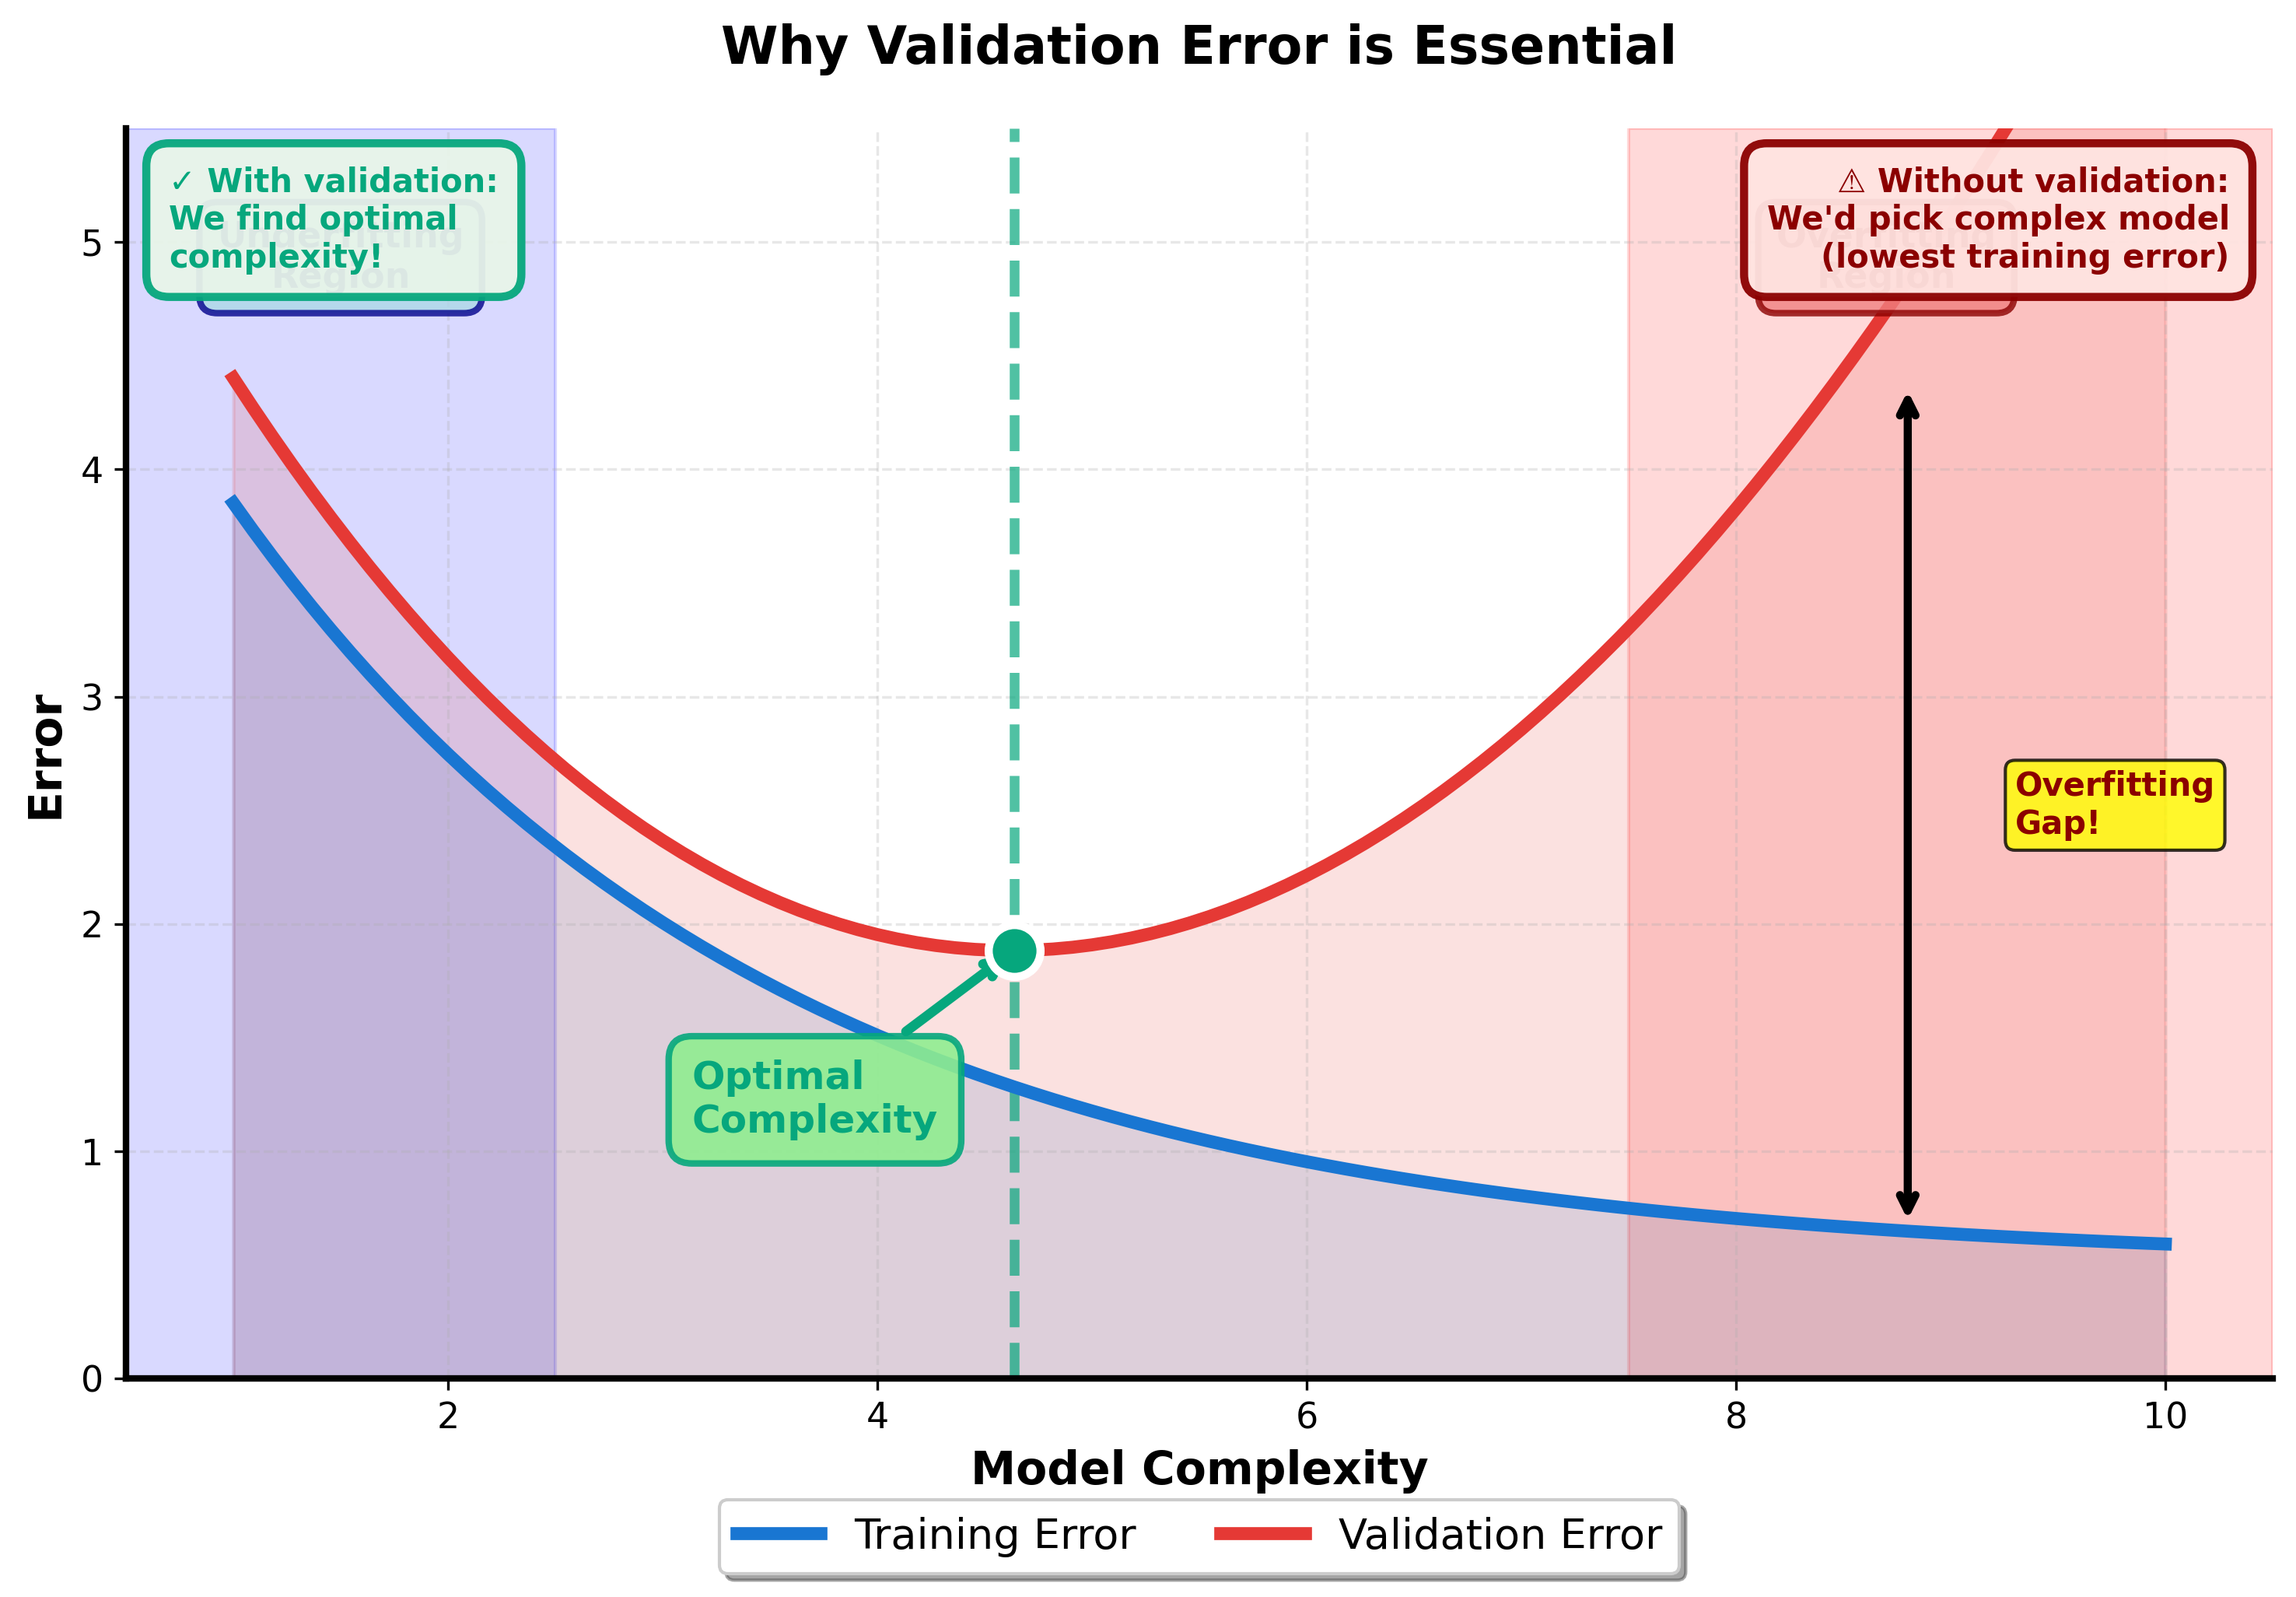
\includegraphics[width=\textwidth]{../figures/validation_necessity.png}
\end{column}
\end{columns}
\end{frame}

\begin{frame}{Learning Curves}
\begin{center}
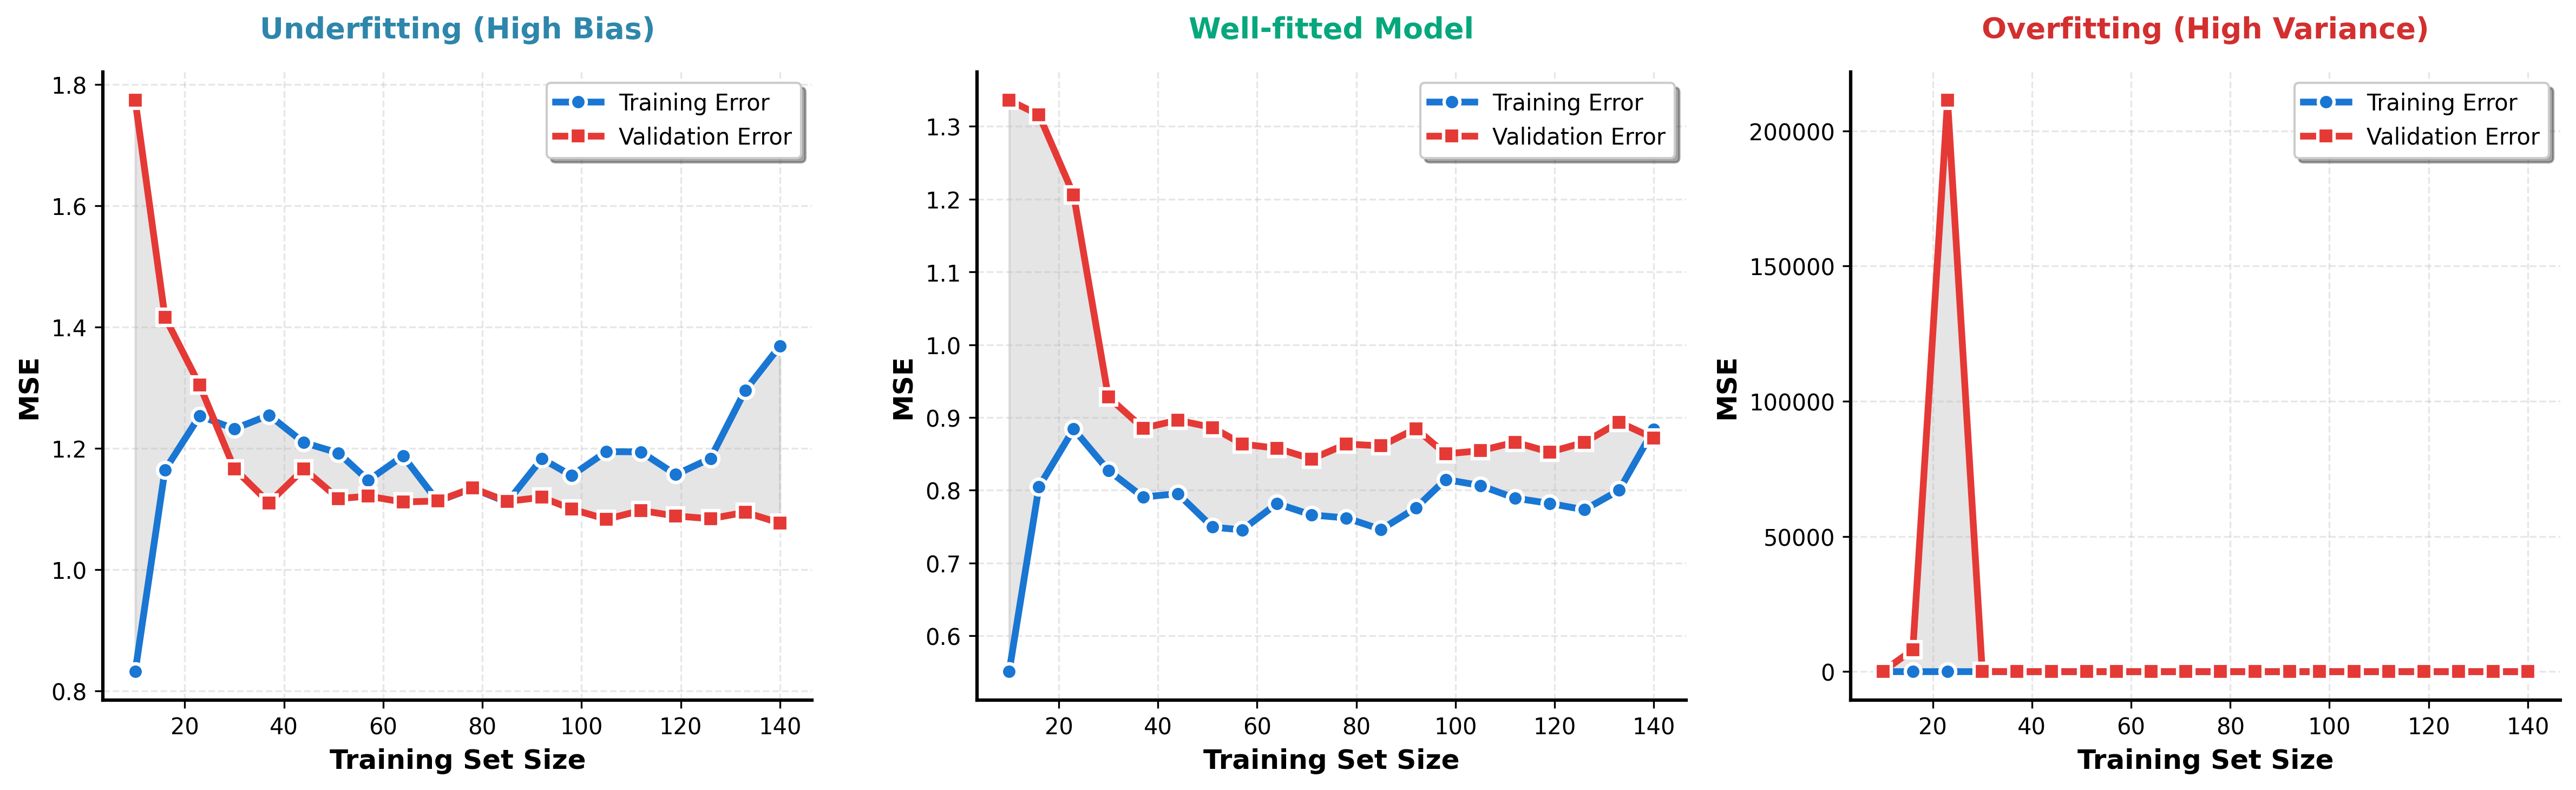
\includegraphics[width=0.95\textwidth]{../figures/learning_curves.png}
\end{center}

\vspace{0.1cm}

\begin{itemize}
\item \textbf{Underfitting:} Both errors high, converge to high value
\item \textbf{Well-fitted:} Both errors low, small gap between them
\item \textbf{Overfitting:} Large gap between training and validation error
\end{itemize}
\end{frame}

\begin{frame}{Cross-Validation: Motivation}
\begin{alertblock}{Problem with Single Train-Val Split}
\begin{itemize}
\setlength{\itemsep}{2pt}
\item Results depend on random split
\item Some data points never used for training
\item Some never used for validation
\item High variance in performance estimates
\end{itemize}
\end{alertblock}

\vspace{0.2cm}

\begin{exampleblock}{Cross-Validation Solution}
\begin{itemize}
\setlength{\itemsep}{2pt}
\item Use multiple train-validation splits
\item Every data point used for both training and validation
\item Average results across splits for robust estimate
\item Reduces variance in performance evaluation
\end{itemize}
\end{exampleblock}
\end{frame}

\begin{frame}{Cross-Validation Schemes}
\begin{center}
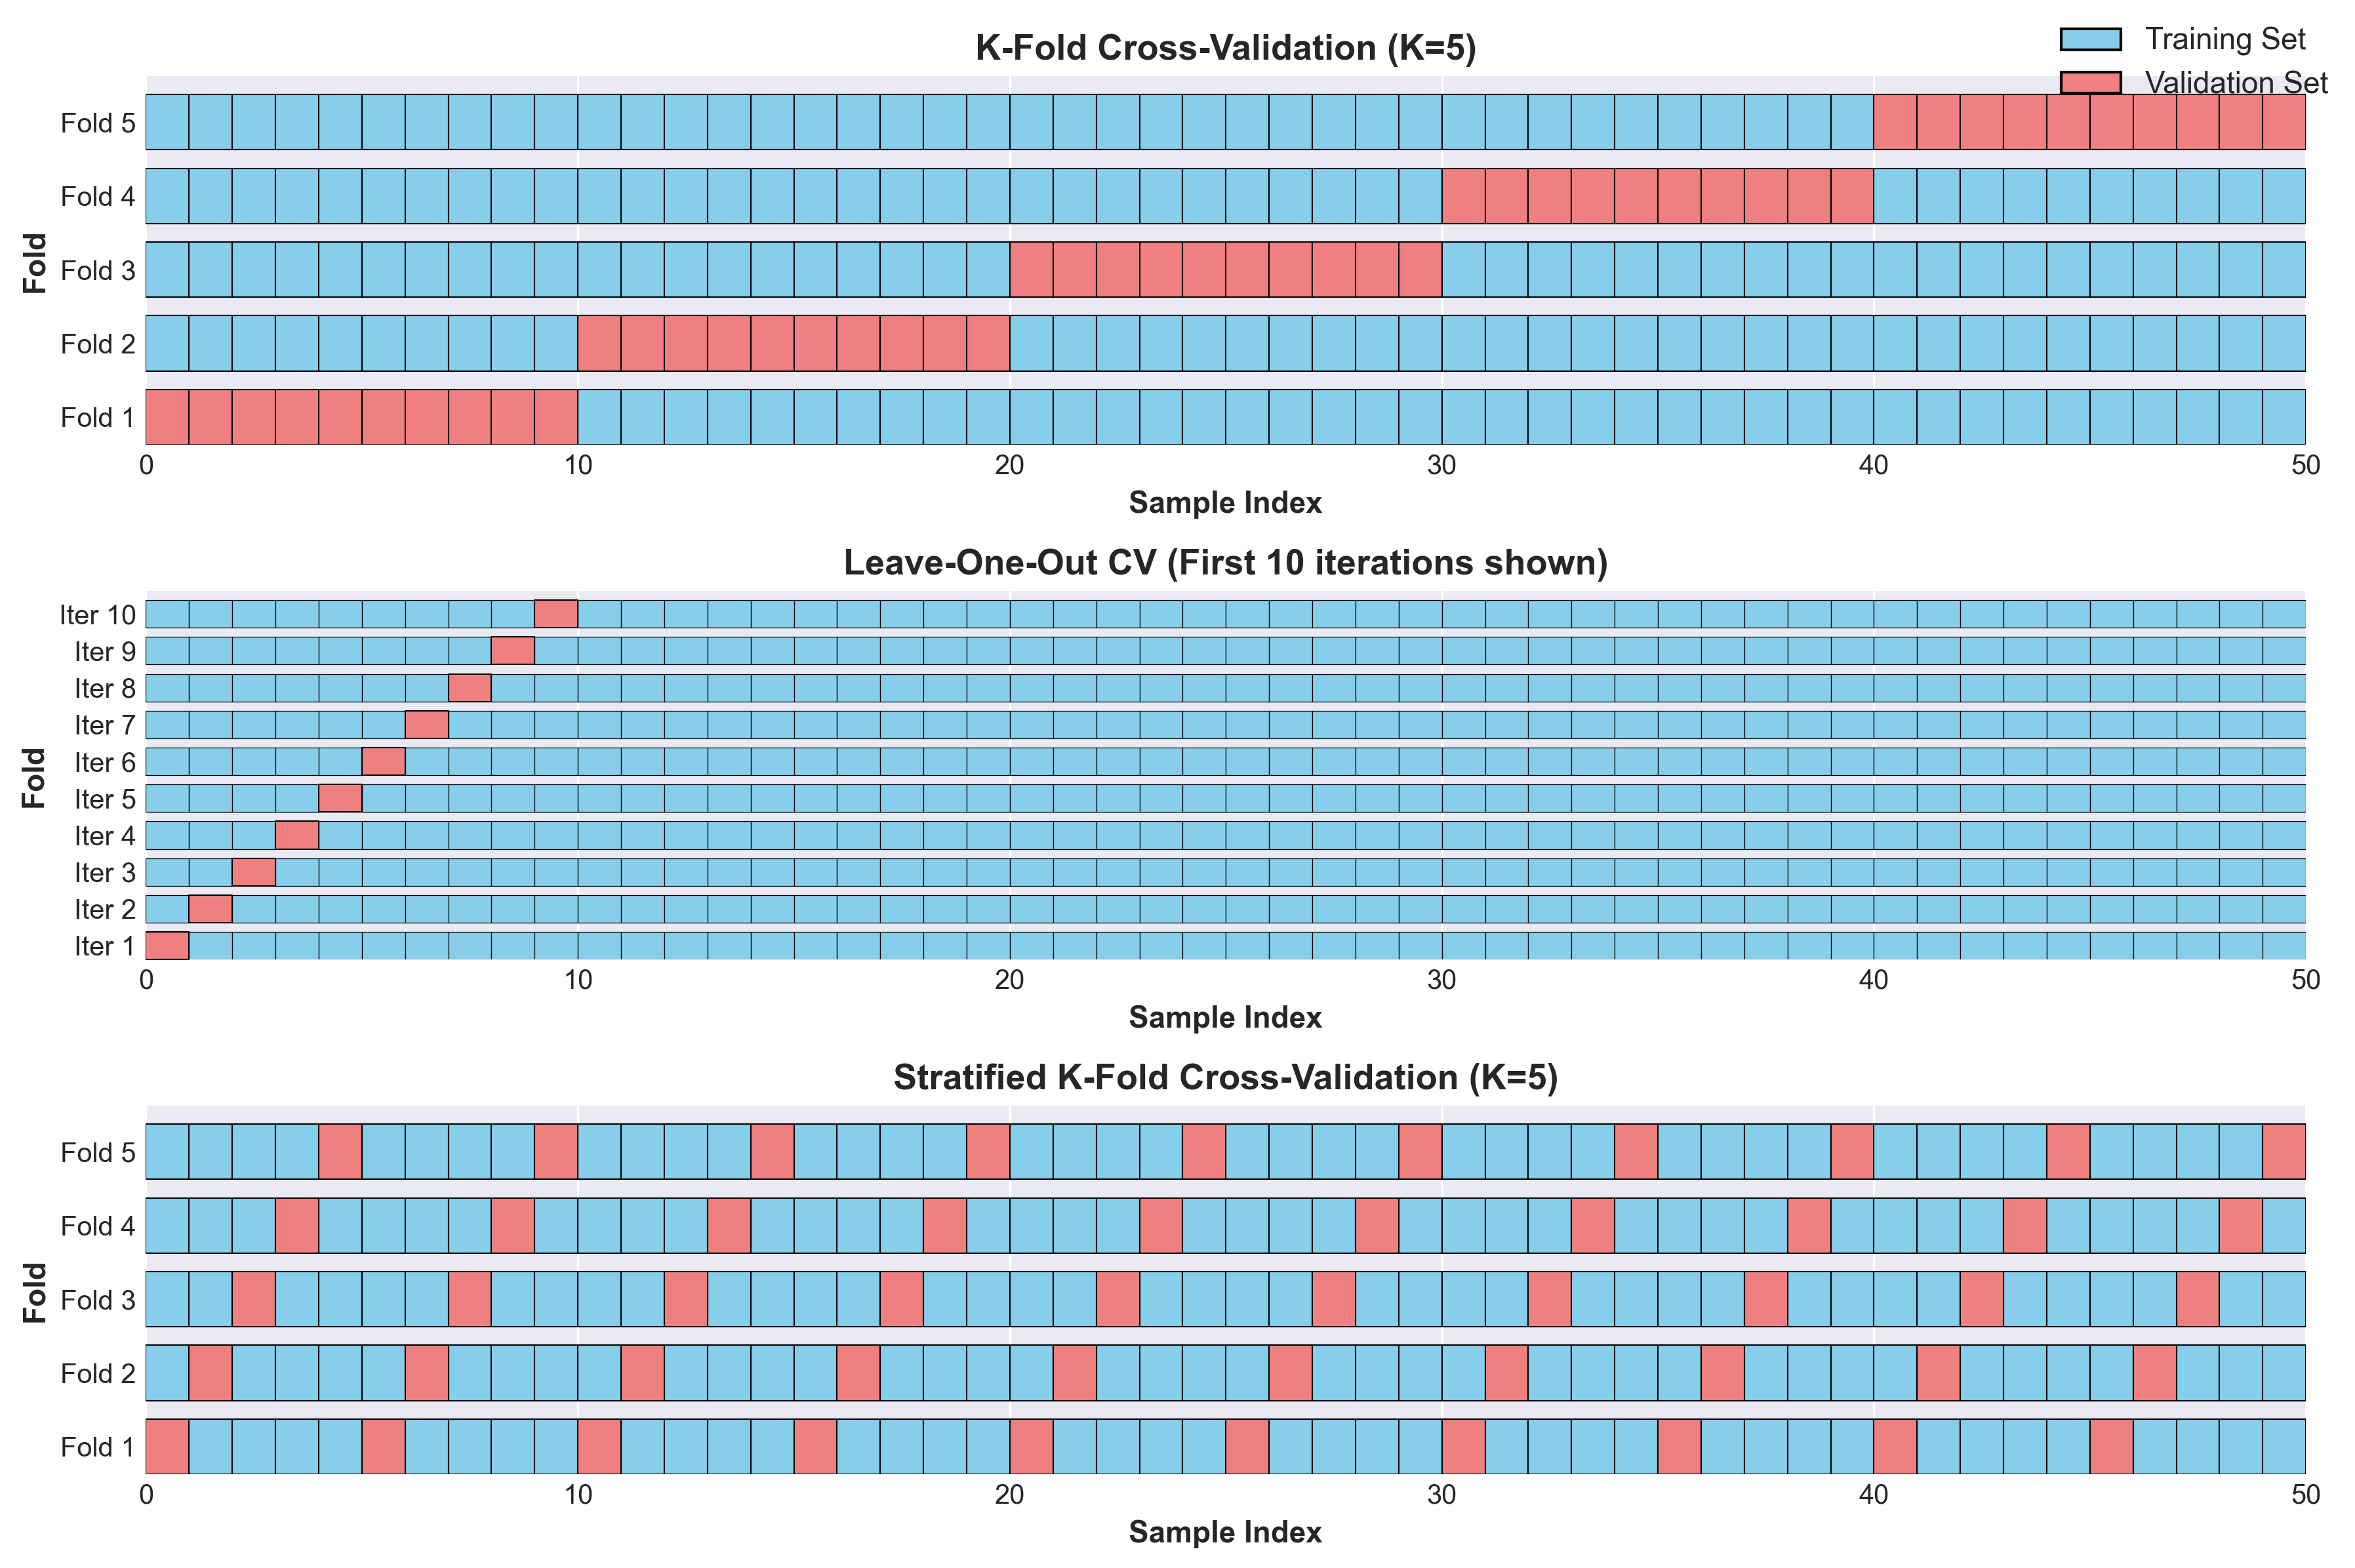
\includegraphics[width=0.85\textwidth]{../figures/cross_validation_schemes.png}
\end{center}

\vspace{0.1cm}

\begin{columns}[t]
\begin{column}{0.48\textwidth}
\begin{block}{K-Fold CV}
\begin{itemize}
\setlength{\itemsep}{1pt}
\item Split data into K folds
\item Train on K-1, validate on 1
\item Repeat K times
\item Average K results
\end{itemize}
\end{block}
\end{column}

\begin{column}{0.48\textwidth}
\begin{block}{Stratified K-Fold}
\begin{itemize}
\setlength{\itemsep}{1pt}
\item Maintains class distribution
\item Important for imbalanced data
\item Each fold representative
\item Same averaging as K-Fold
\end{itemize}
\end{block}
\end{column}
\end{columns}
\end{frame}

\begin{frame}{K-Fold Cross-Validation Algorithm}
\begin{algorithm}[H]
\caption{K-Fold Cross-Validation}
\begin{algorithmic}[1]
\REQUIRE Dataset $D$, Model $M$, Number of folds $K$
\ENSURE Cross-validation score
\STATE Randomly partition $D$ into $K$ equal-sized subsets $D_1, D_2, \ldots, D_K$
\STATE Initialize $\text{scores} = []$
\FOR{$i = 1$ to $K$}
    \STATE $D_{\text{val}} \leftarrow D_i$
    \STATE $D_{\text{train}} \leftarrow D \setminus D_i$
    \STATE Train model $\hat{M}$ on $D_{\text{train}}$
    \STATE $s_i \leftarrow \text{Evaluate}(\hat{M}, D_{\text{val}})$
    \STATE Append $s_i$ to $\text{scores}$
\ENDFOR
\STATE \textbf{return} $\frac{1}{K} \sum_{i=1}^{K} s_i$
\end{algorithmic}
\end{algorithm}

\vspace{0.1cm}

\begin{tipblock}{Common Choices}
$K = 5$ or $K = 10$ are typical values balancing computational cost and variance reduction.
\end{tipblock}
\end{frame}

\begin{frame}{Validation Curve}
\begin{center}
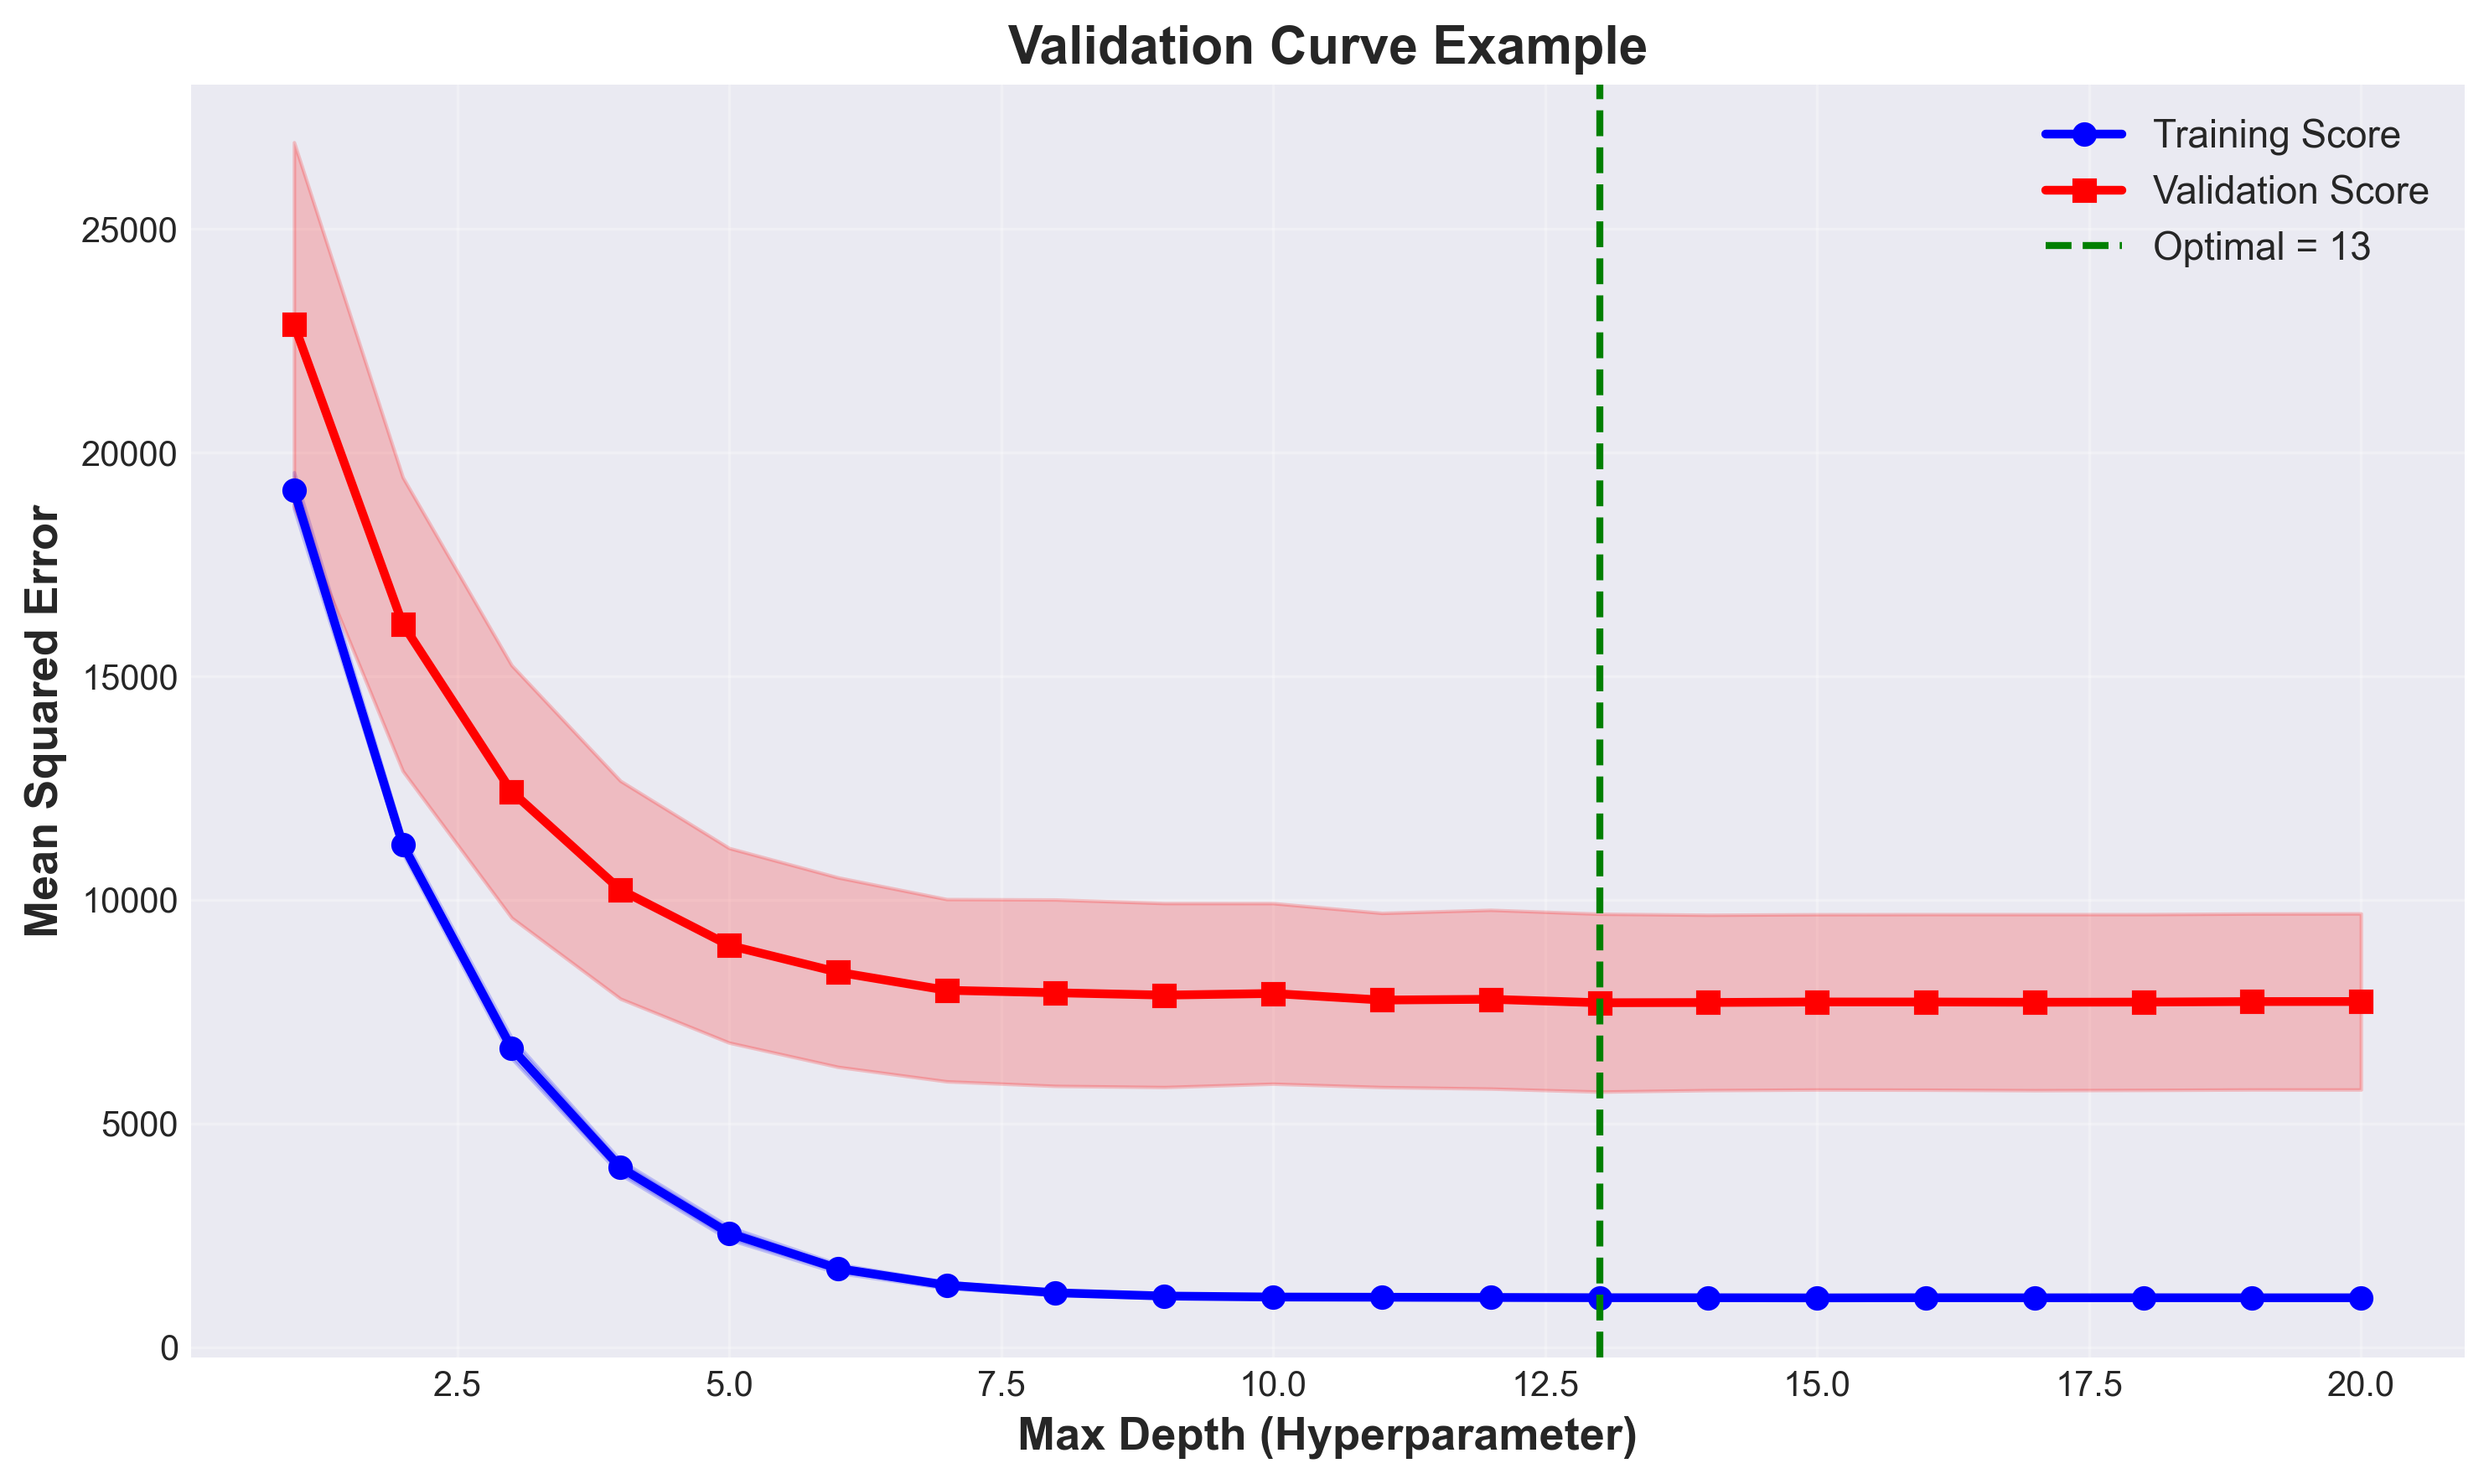
\includegraphics[width=0.75\textwidth]{../figures/validation_curve.png}
\end{center}

\vspace{0.1cm}

\begin{techblock}{Using Validation Curves}
\begin{itemize}
\setlength{\itemsep}{2pt}
\item Plot training and validation scores vs. hyperparameter values
\item Identify optimal hyperparameter setting
\item Diagnose underfitting and overfitting regions
\item Select model with best validation performance
\end{itemize}
\end{techblock}
\end{frame}

% ========================================
% Section: Evaluation Metrics
% ========================================

\section{Evaluation Metrics}

\begin{frame}{Classification Metrics: Confusion Matrix}
\begin{columns}[t]
\begin{column}{0.52\textwidth}
\begin{center}
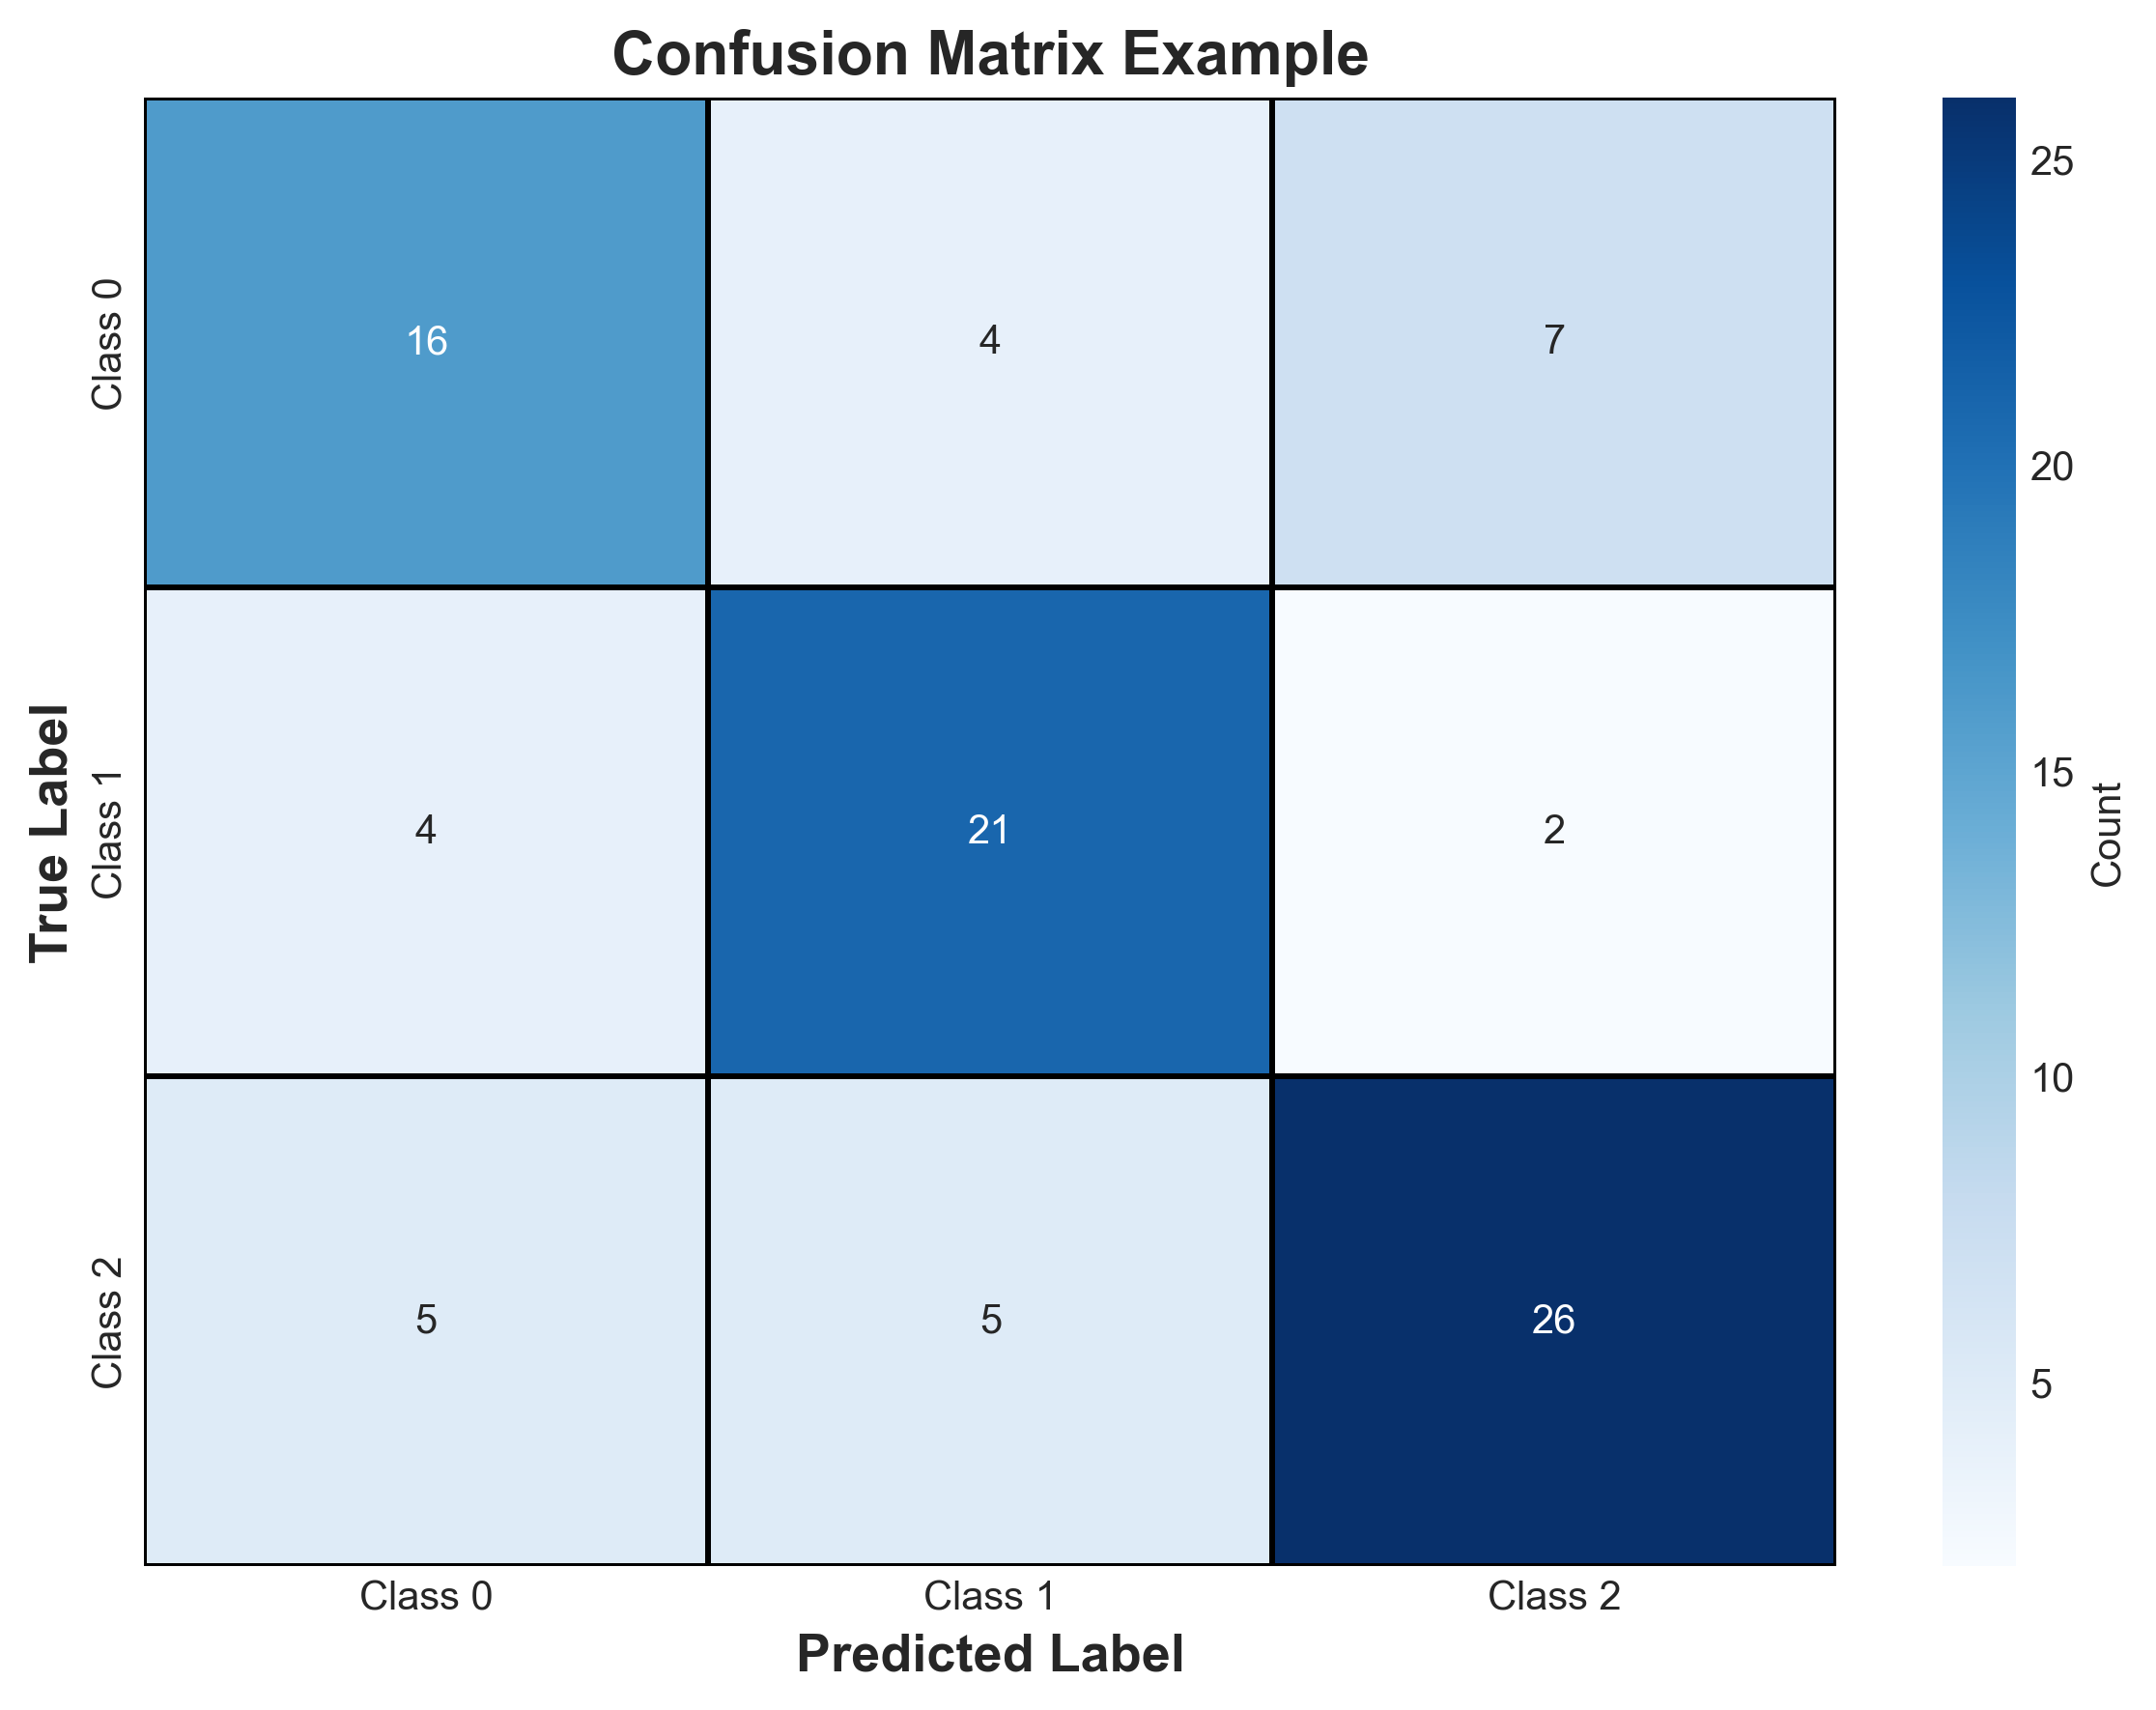
\includegraphics[width=\textwidth]{../figures/confusion_matrix.png}
\end{center}
\end{column}

\begin{column}{0.44\textwidth}
\vspace{0.3cm}
\begin{block}{Definitions}
\begin{itemize}
\setlength{\itemsep}{1pt}
\item \textbf{TP:} True Positives
\item \textbf{TN:} True Negatives
\item \textbf{FP:} False Positives (Type I error)
\item \textbf{FN:} False Negatives (Type II error)
\end{itemize}
\end{block}

\vspace{0.1cm}

\begin{alertblock}{Key Metrics}
\vspace{-0.1cm}
\begin{align*}
\text{Accuracy} &= \frac{TP + TN}{TP + TN + FP + FN} \\
\text{Precision} &= \frac{TP}{TP + FP} \\
\text{Recall} &= \frac{TP}{TP + FN}
\end{align*}
\end{alertblock}
\end{column}
\end{columns}
\end{frame}

\begin{frame}{Classification Metrics Comparison}
\begin{center}
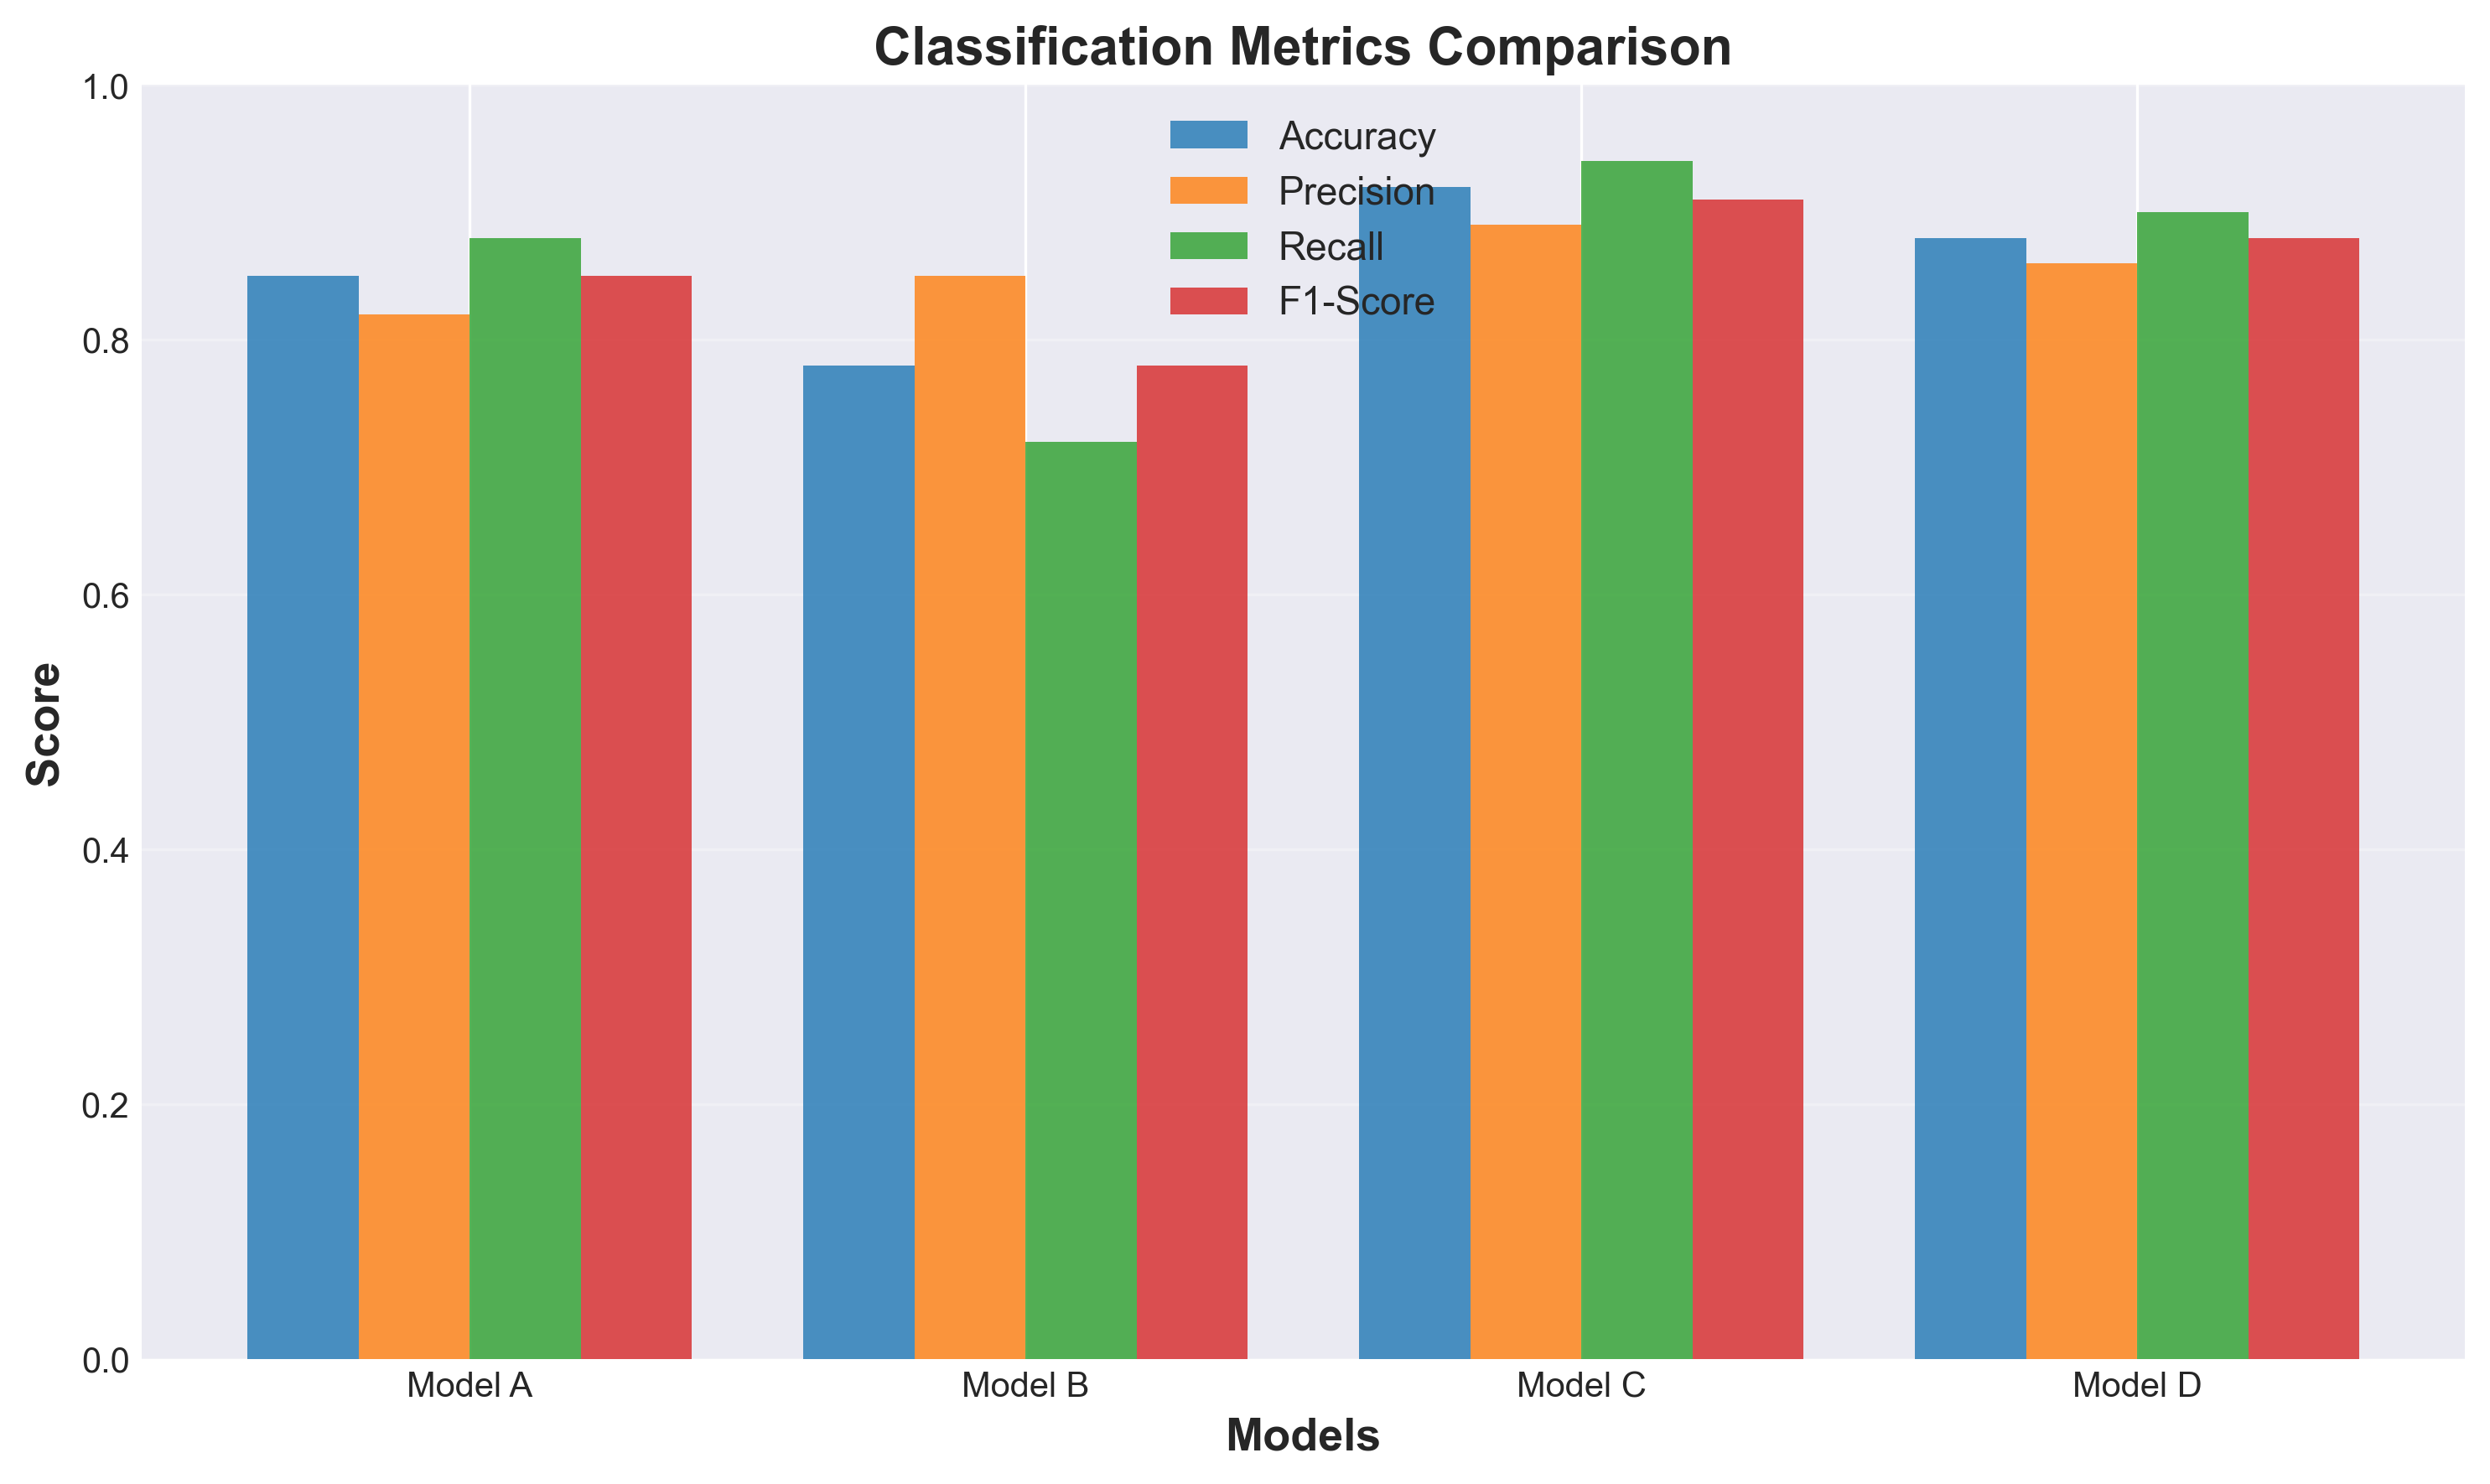
\includegraphics[width=0.8\textwidth]{../figures/metrics_comparison.png}
\end{center}

\vspace{0.1cm}

\begin{columns}[t]
\begin{column}{0.48\textwidth}
\begin{block}{Accuracy}
Overall correctness; can be misleading with imbalanced classes
\end{block}
\end{column}

\begin{column}{0.48\textwidth}
\begin{block}{F1-Score}
Harmonic mean of precision and recall: $F_1 = \frac{2 \cdot \text{Precision} \cdot \text{Recall}}{\text{Precision} + \text{Recall}}$
\end{block}
\end{column}
\end{columns}
\end{frame}

\begin{frame}{ROC Curve and AUC}
\begin{columns}[t]
\begin{column}{0.55\textwidth}
\begin{center}
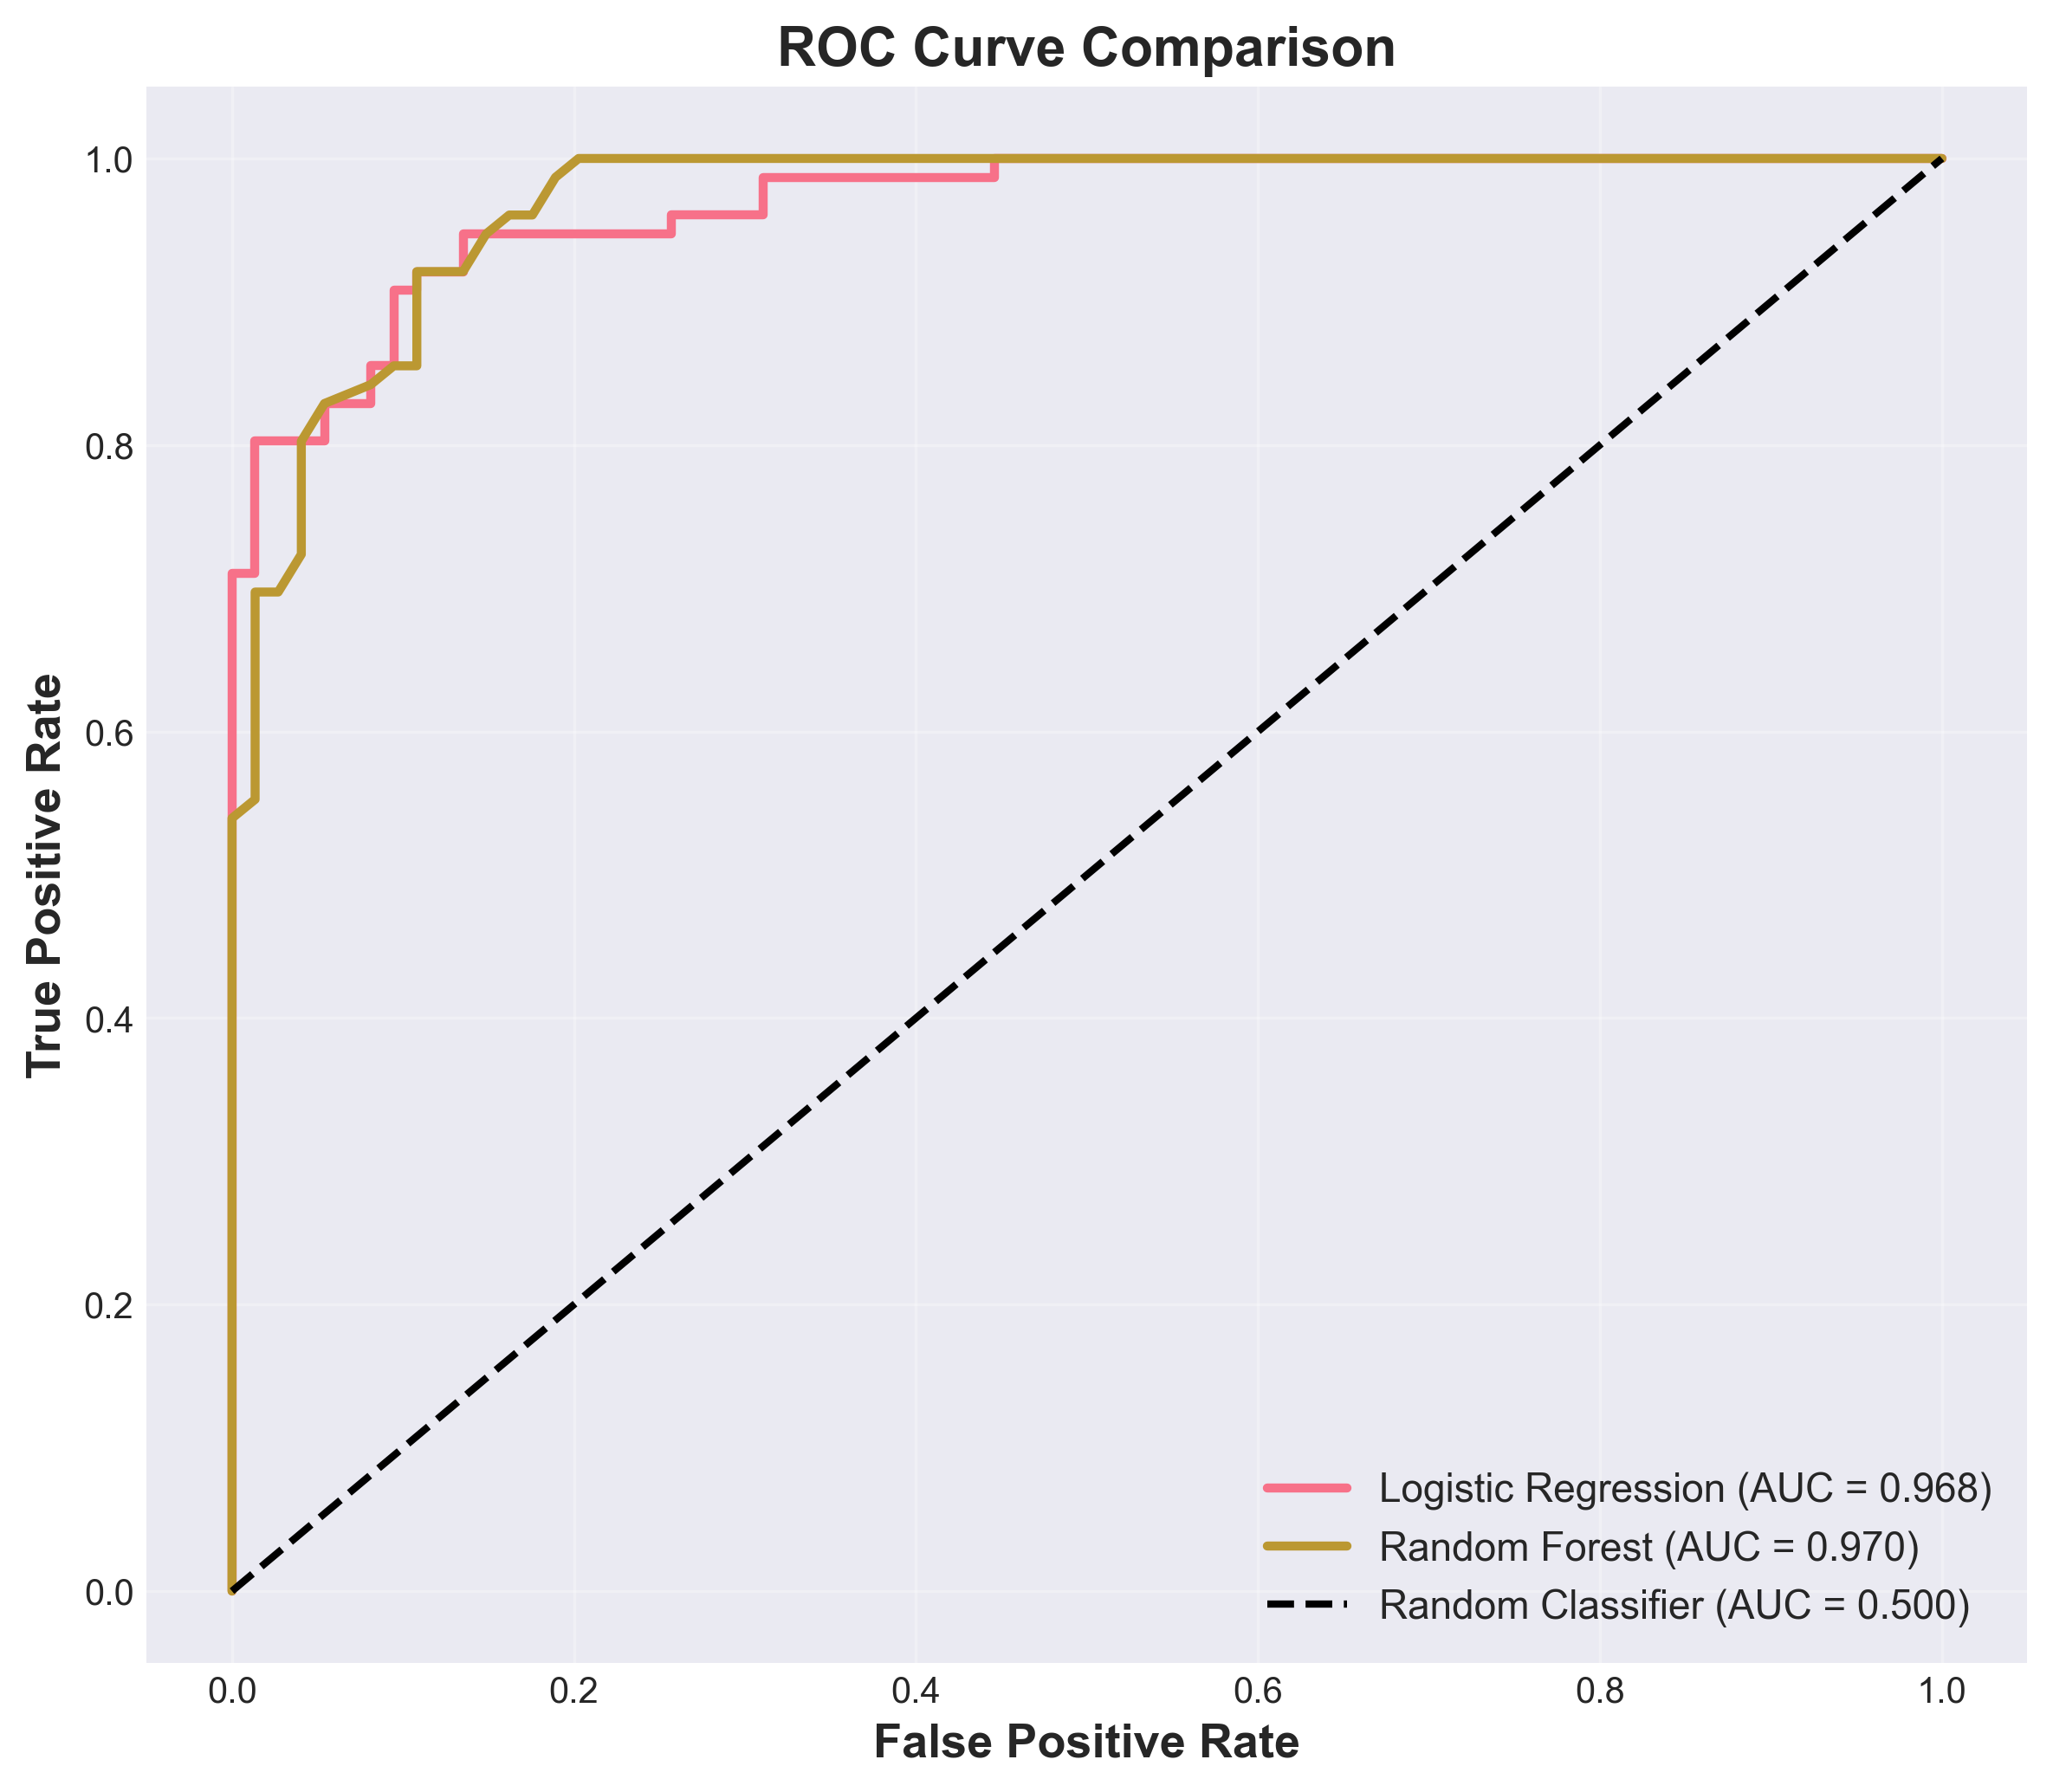
\includegraphics[width=\textwidth]{../figures/roc_curve.png}
\end{center}
\end{column}

\begin{column}{0.42\textwidth}
\begin{block}{ROC Curve}
\begin{itemize}
\setlength{\itemsep}{2pt}
\item Plots TPR vs FPR
\item Shows performance across thresholds
\item Diagonal = random classifier
\item Upper-left corner = perfect
\end{itemize}
\end{block}

\vspace{0.1cm}

\begin{exampleblock}{AUC Score}
\begin{itemize}
\setlength{\itemsep}{2pt}
\item Area Under ROC Curve
\item Range: [0, 1]
\item 0.5 = random
\item 1.0 = perfect
\item Threshold-independent
\end{itemize}
\end{exampleblock}
\end{column}
\end{columns}
\end{frame}

\begin{frame}{Precision-Recall Curve}
\begin{columns}[t]
\begin{column}{0.55\textwidth}
\begin{center}
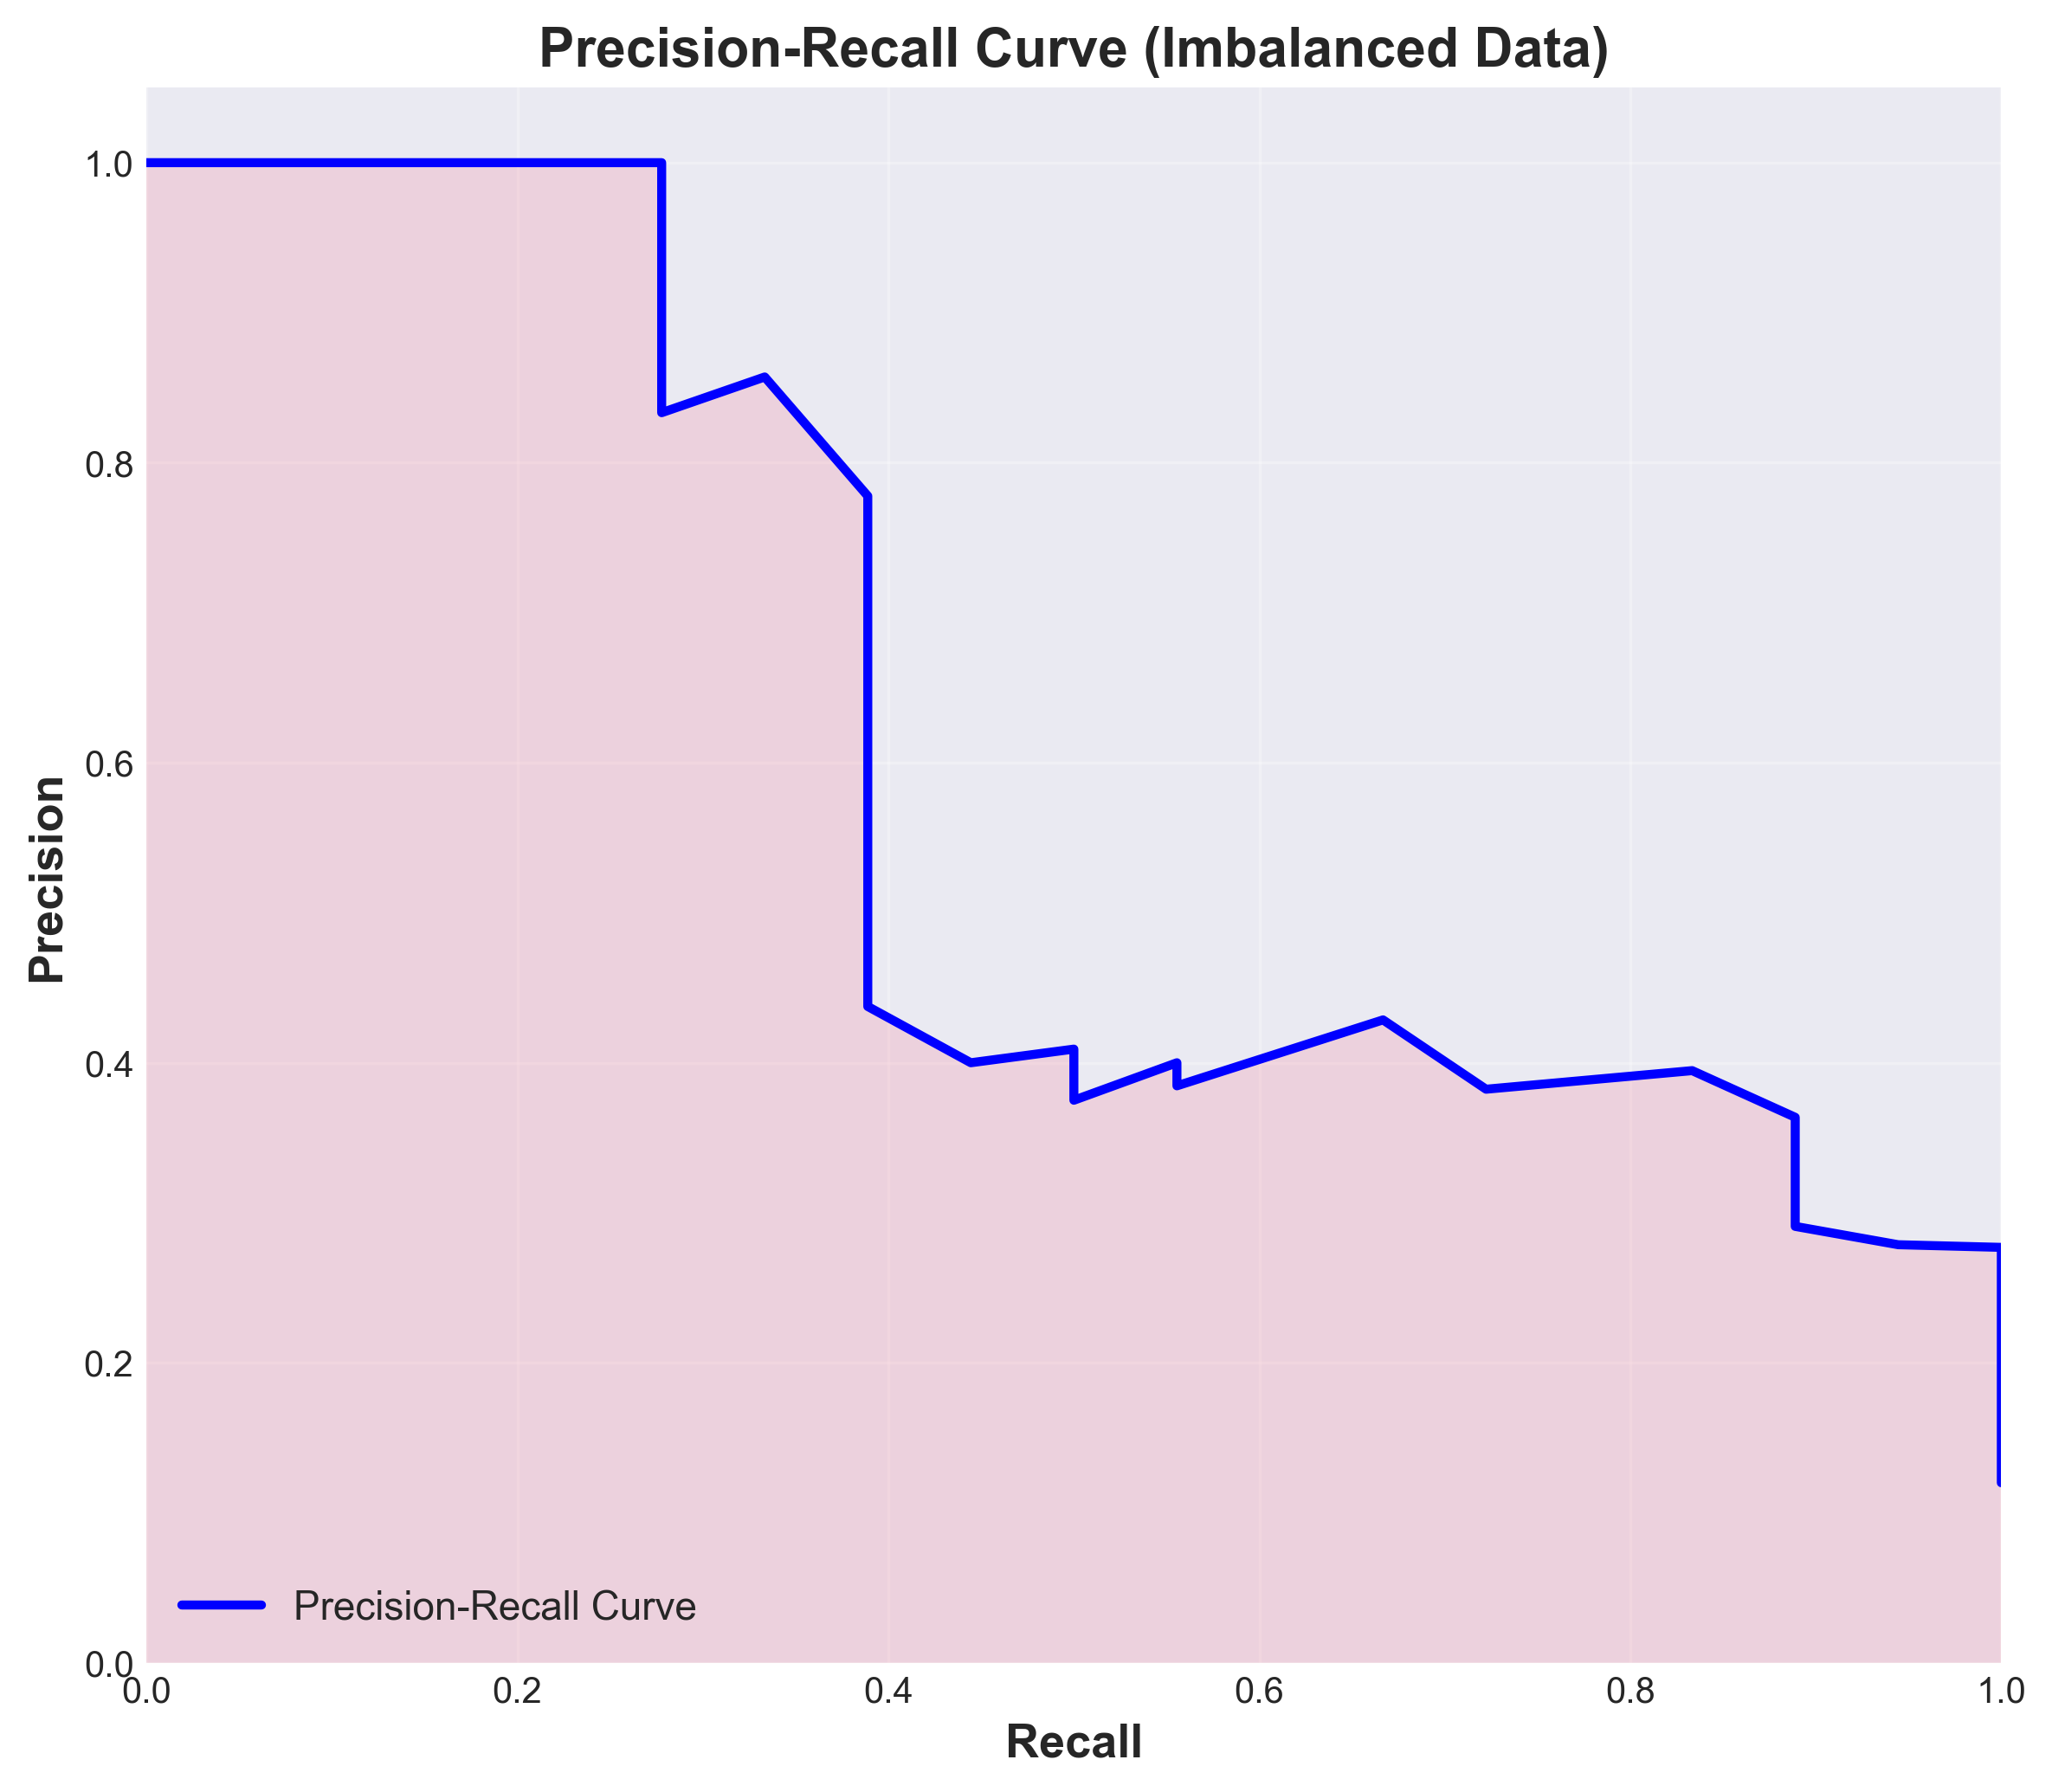
\includegraphics[width=\textwidth]{../figures/precision_recall_curve.png}
\end{center}
\end{column}

\begin{column}{0.42\textwidth}
\begin{alertblock}{When to Use}
\begin{itemize}
\setlength{\itemsep}{2pt}
\item Imbalanced datasets
\item Care about positive class
\item False positives costly
\item Alternative to ROC
\end{itemize}
\end{alertblock}

\vspace{0.1cm}

\begin{tipblock}{Interpretation}
\begin{itemize}
\setlength{\itemsep}{2pt}
\item High area = good performance
\item Trade-off between precision and recall
\item Choose threshold based on application needs
\end{itemize}
\end{tipblock}
\end{column}
\end{columns}
\end{frame}

\begin{frame}{Regression Metrics}
\begin{columns}[t]
\begin{column}{0.48\textwidth}
\begin{block}{Mean Squared Error (MSE)}
\vspace{-0.1cm}
\begin{equation*}
\text{MSE} = \frac{1}{n}\sum_{i=1}^{n}(y_i - \hat{y}_i)^2
\end{equation*}
\begin{itemize}
\setlength{\itemsep}{1pt}
\item Penalizes large errors heavily
\item Same units as $y^2$
\item Always non-negative
\item Lower is better
\end{itemize}
\end{block}

\vspace{0.1cm}

\begin{block}{Root Mean Squared Error}
\vspace{-0.1cm}
\begin{equation*}
\text{RMSE} = \sqrt{\text{MSE}}
\end{equation*}
\begin{itemize}
\setlength{\itemsep}{1pt}
\item Same units as $y$
\item More interpretable than MSE
\end{itemize}
\end{block}
\end{column}

\begin{column}{0.48\textwidth}
\begin{block}{Mean Absolute Error (MAE)}
\vspace{-0.1cm}
\begin{equation*}
\text{MAE} = \frac{1}{n}\sum_{i=1}^{n}|y_i - \hat{y}_i|
\end{equation*}
\begin{itemize}
\setlength{\itemsep}{1pt}
\item Robust to outliers
\item Same units as $y$
\item Easy to interpret
\end{itemize}
\end{block}

\vspace{0.1cm}

\begin{block}{R-Squared ($R^2$)}
\vspace{-0.1cm}
\begin{equation*}
R^2 = 1 - \frac{\sum(y_i - \hat{y}_i)^2}{\sum(y_i - \bar{y})^2}
\end{equation*}
\begin{itemize}
\setlength{\itemsep}{1pt}
\item Proportion of variance explained
\item Range: $(-\infty, 1]$
\item 1 = perfect predictions
\end{itemize}
\end{block}
\end{column}
\end{columns}
\end{frame}

% ========================================
% Section: Regularization
% ========================================

\section{Regularization}

\begin{frame}{What is Regularization?}
\begin{alertblock}{Definition}
Regularization is a technique to prevent overfitting by adding a penalty term to the loss function that discourages complex models.
\end{alertblock}

\vspace{0.2cm}

\begin{exampleblock}{General Form}
\begin{equation*}
\text{Loss}_{\text{regularized}} = \text{Loss}_{\text{data}} + \lambda \cdot \text{Penalty}(\text{parameters})
\end{equation*}
where $\lambda \geq 0$ is the \textbf{regularization parameter} controlling the strength of regularization.
\end{exampleblock}

\vspace{0.2cm}

\begin{columns}[t]
\begin{column}{0.48\textwidth}
\begin{block}{Benefits}
\begin{itemize}
\setlength{\itemsep}{2pt}
\item Reduces overfitting
\item Improves generalization
\item Encourages simpler models
\item Can perform feature selection
\end{itemize}
\end{block}
\end{column}

\begin{column}{0.48\textwidth}
\begin{block}{Trade-off}
\begin{itemize}
\setlength{\itemsep}{2pt}
\item $\lambda$ too small: underfitting
\item $\lambda$ too large: underfitting
\item Must tune $\lambda$ via validation
\end{itemize}
\end{block}
\end{column}
\end{columns}
\end{frame}

\begin{frame}{Ridge Regression (L2 Regularization)}
\begin{columns}[t]
\begin{column}{0.58\textwidth}
\begin{block}{Objective Function}
\vspace{-0.1cm}
\begin{equation*}
\min_{\mathbf{w}} \sum_{i=1}^{n}(y_i - \mathbf{w}^T\mathbf{x}_i)^2 + \lambda \|\mathbf{w}\|_2^2
\end{equation*}
where $\|\mathbf{w}\|_2^2 = \sum_{j=1}^{d} w_j^2$ is the L2 norm.
\end{block}

\vspace{0.1cm}

\begin{exampleblock}{Characteristics}
\begin{itemize}
\setlength{\itemsep}{2pt}
\item Shrinks coefficients towards zero
\item Does not set coefficients exactly to zero
\item Has closed-form solution
\item Stable and computationally efficient
\item Preferred when all features are relevant
\end{itemize}
\end{exampleblock}

\vspace{0.1cm}

\begin{block}{Solution}
\vspace{-0.1cm}
\begin{equation*}
\hat{\mathbf{w}} = (\mathbf{X}^T\mathbf{X} + \lambda \mathbf{I})^{-1}\mathbf{X}^T\mathbf{y}
\end{equation*}
\end{block}
\end{column}

\begin{column}{0.38\textwidth}
\begin{center}
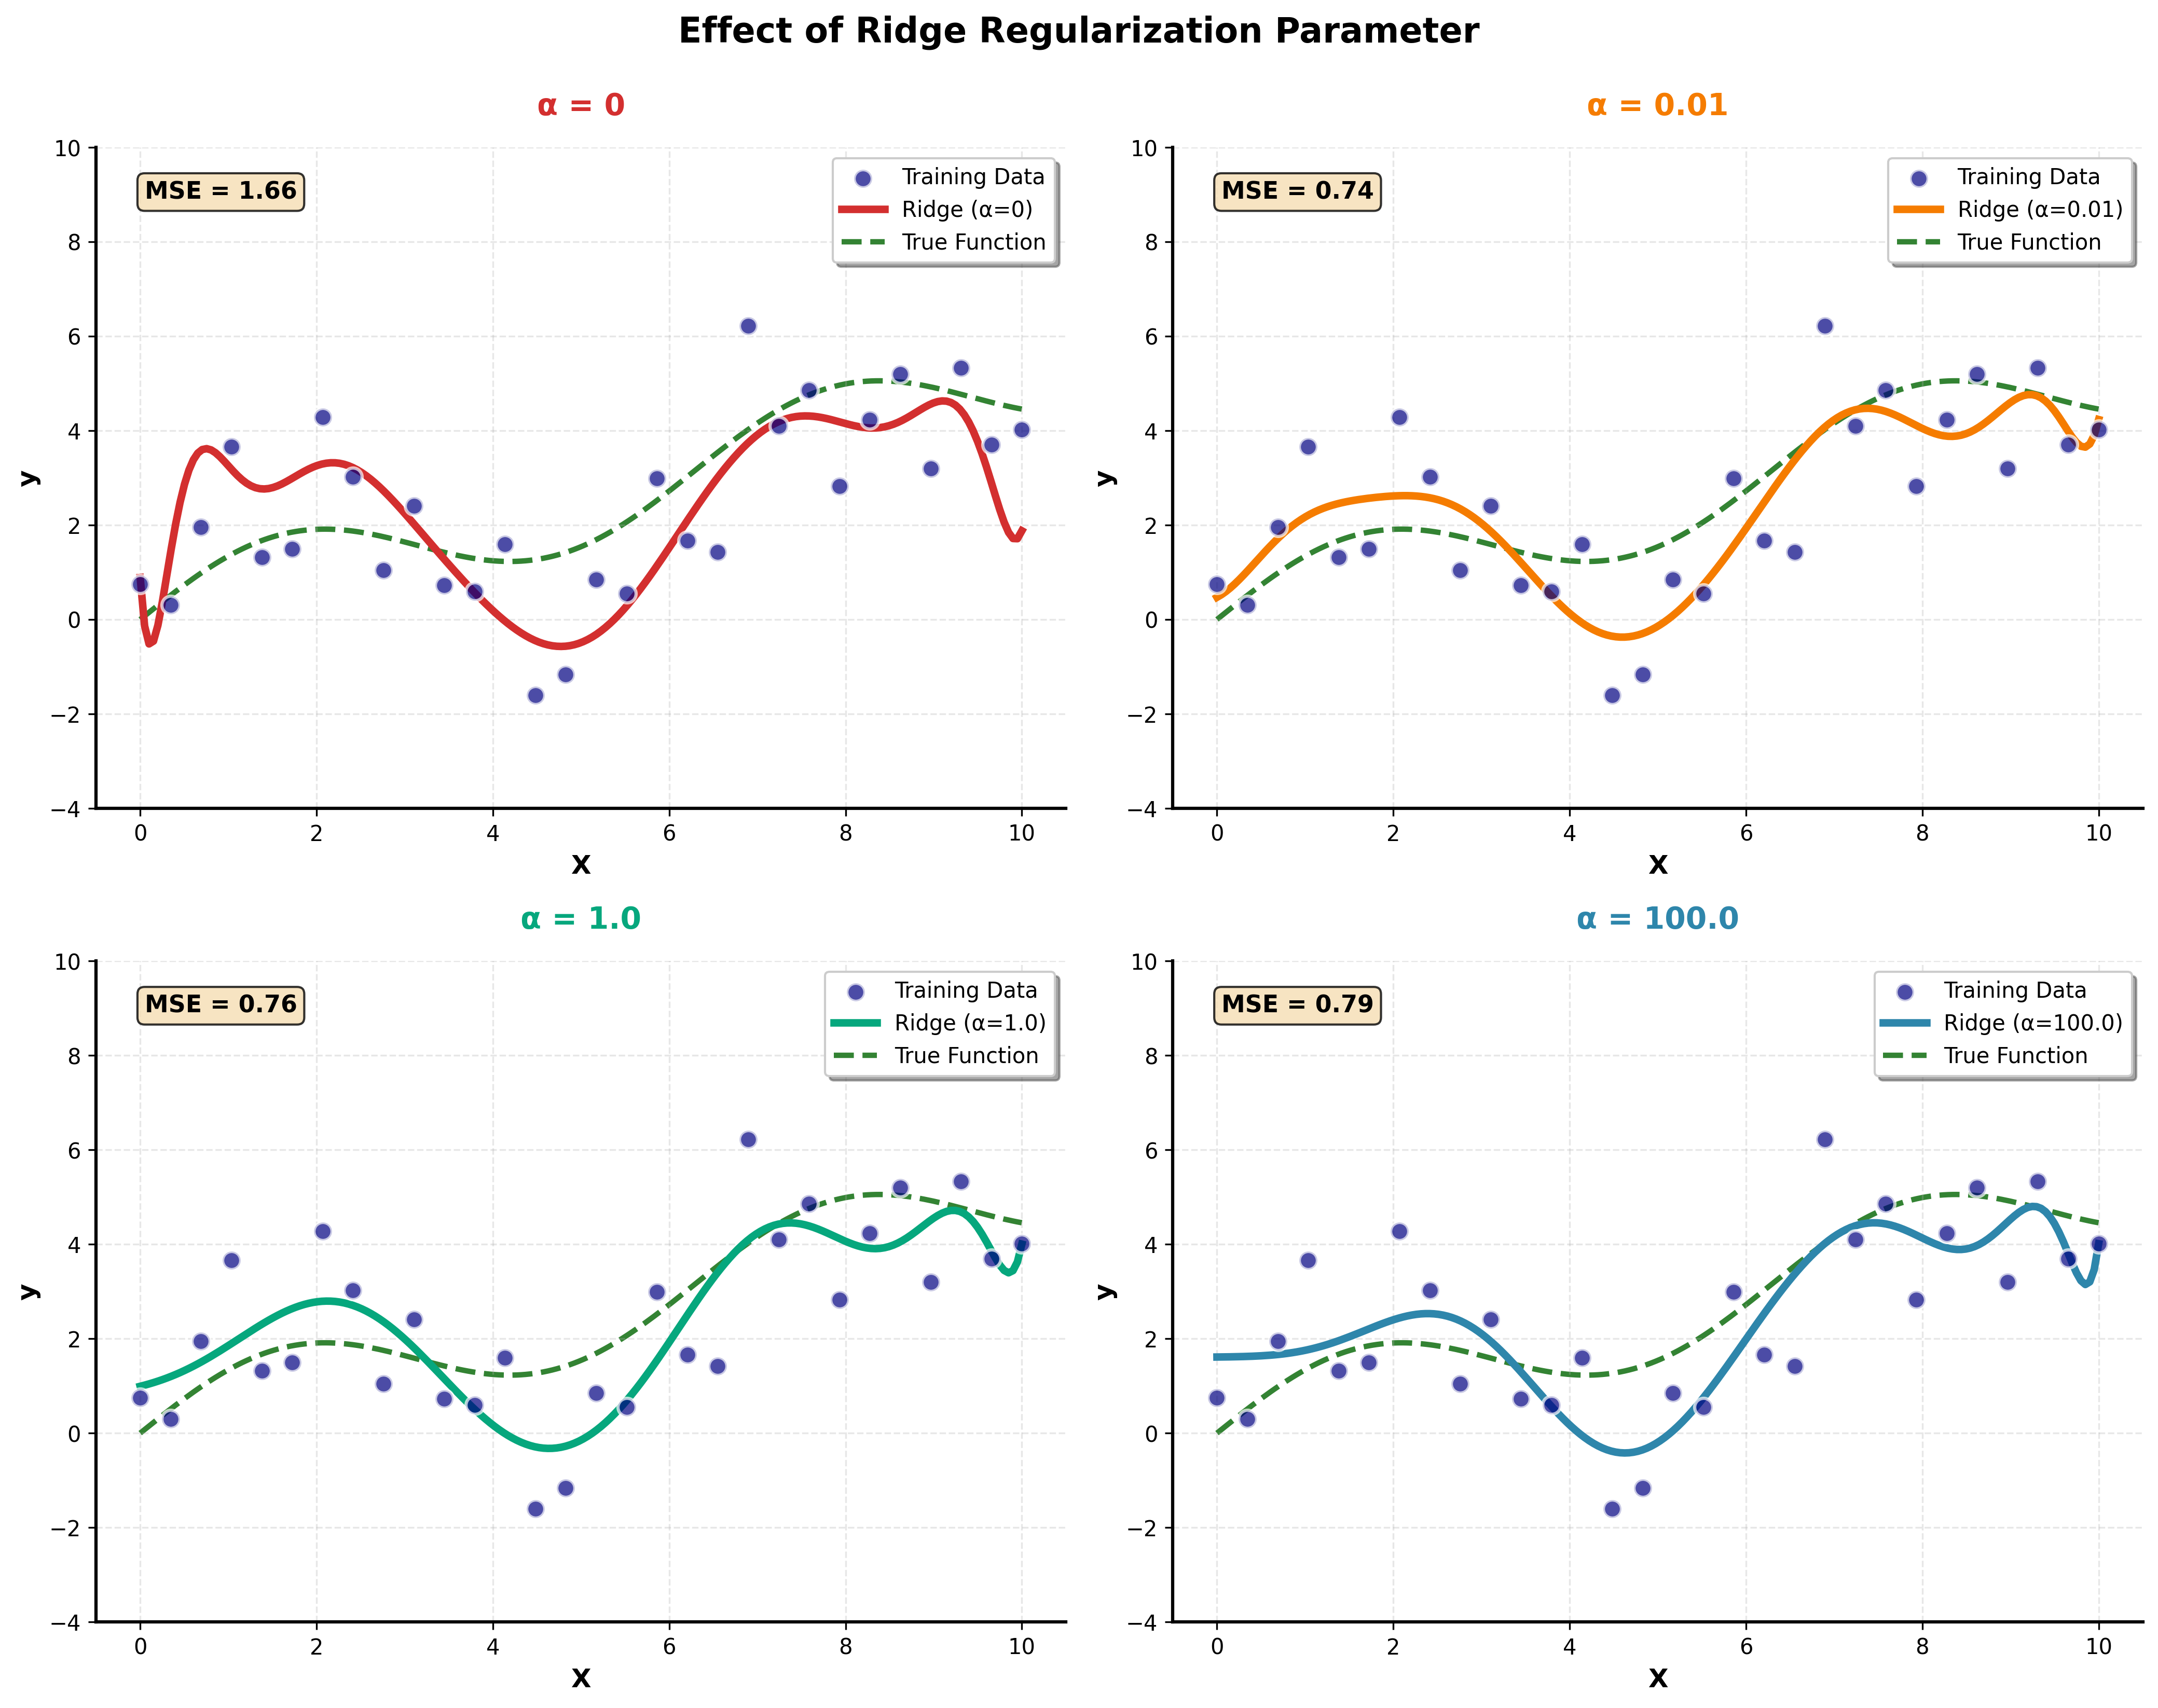
\includegraphics[width=\textwidth]{../figures/regularization_effect.png}
\end{center}
\end{column}
\end{columns}
\end{frame}

\begin{frame}{Lasso Regression (L1 Regularization)}
\begin{columns}[t]
\begin{column}{0.58\textwidth}
\begin{block}{Objective Function}
\vspace{-0.1cm}
\begin{equation*}
\min_{\mathbf{w}} \sum_{i=1}^{n}(y_i - \mathbf{w}^T\mathbf{x}_i)^2 + \lambda \|\mathbf{w}\|_1
\end{equation*}
where $\|\mathbf{w}\|_1 = \sum_{j=1}^{d} |w_j|$ is the L1 norm.
\end{block}

\vspace{0.1cm}

\begin{exampleblock}{Characteristics}
\begin{itemize}
\setlength{\itemsep}{2pt}
\item Can set coefficients exactly to zero
\item Performs automatic feature selection
\item Produces sparse models
\item No closed-form solution (use optimization)
\item Preferred with many irrelevant features
\end{itemize}
\end{exampleblock}

\vspace{0.1cm}

\begin{alertblock}{Sparsity Property}
Lasso's ability to zero out coefficients makes it ideal for interpretable models and high-dimensional data.
\end{alertblock}
\end{column}

\begin{column}{0.38\textwidth}
\begin{center}
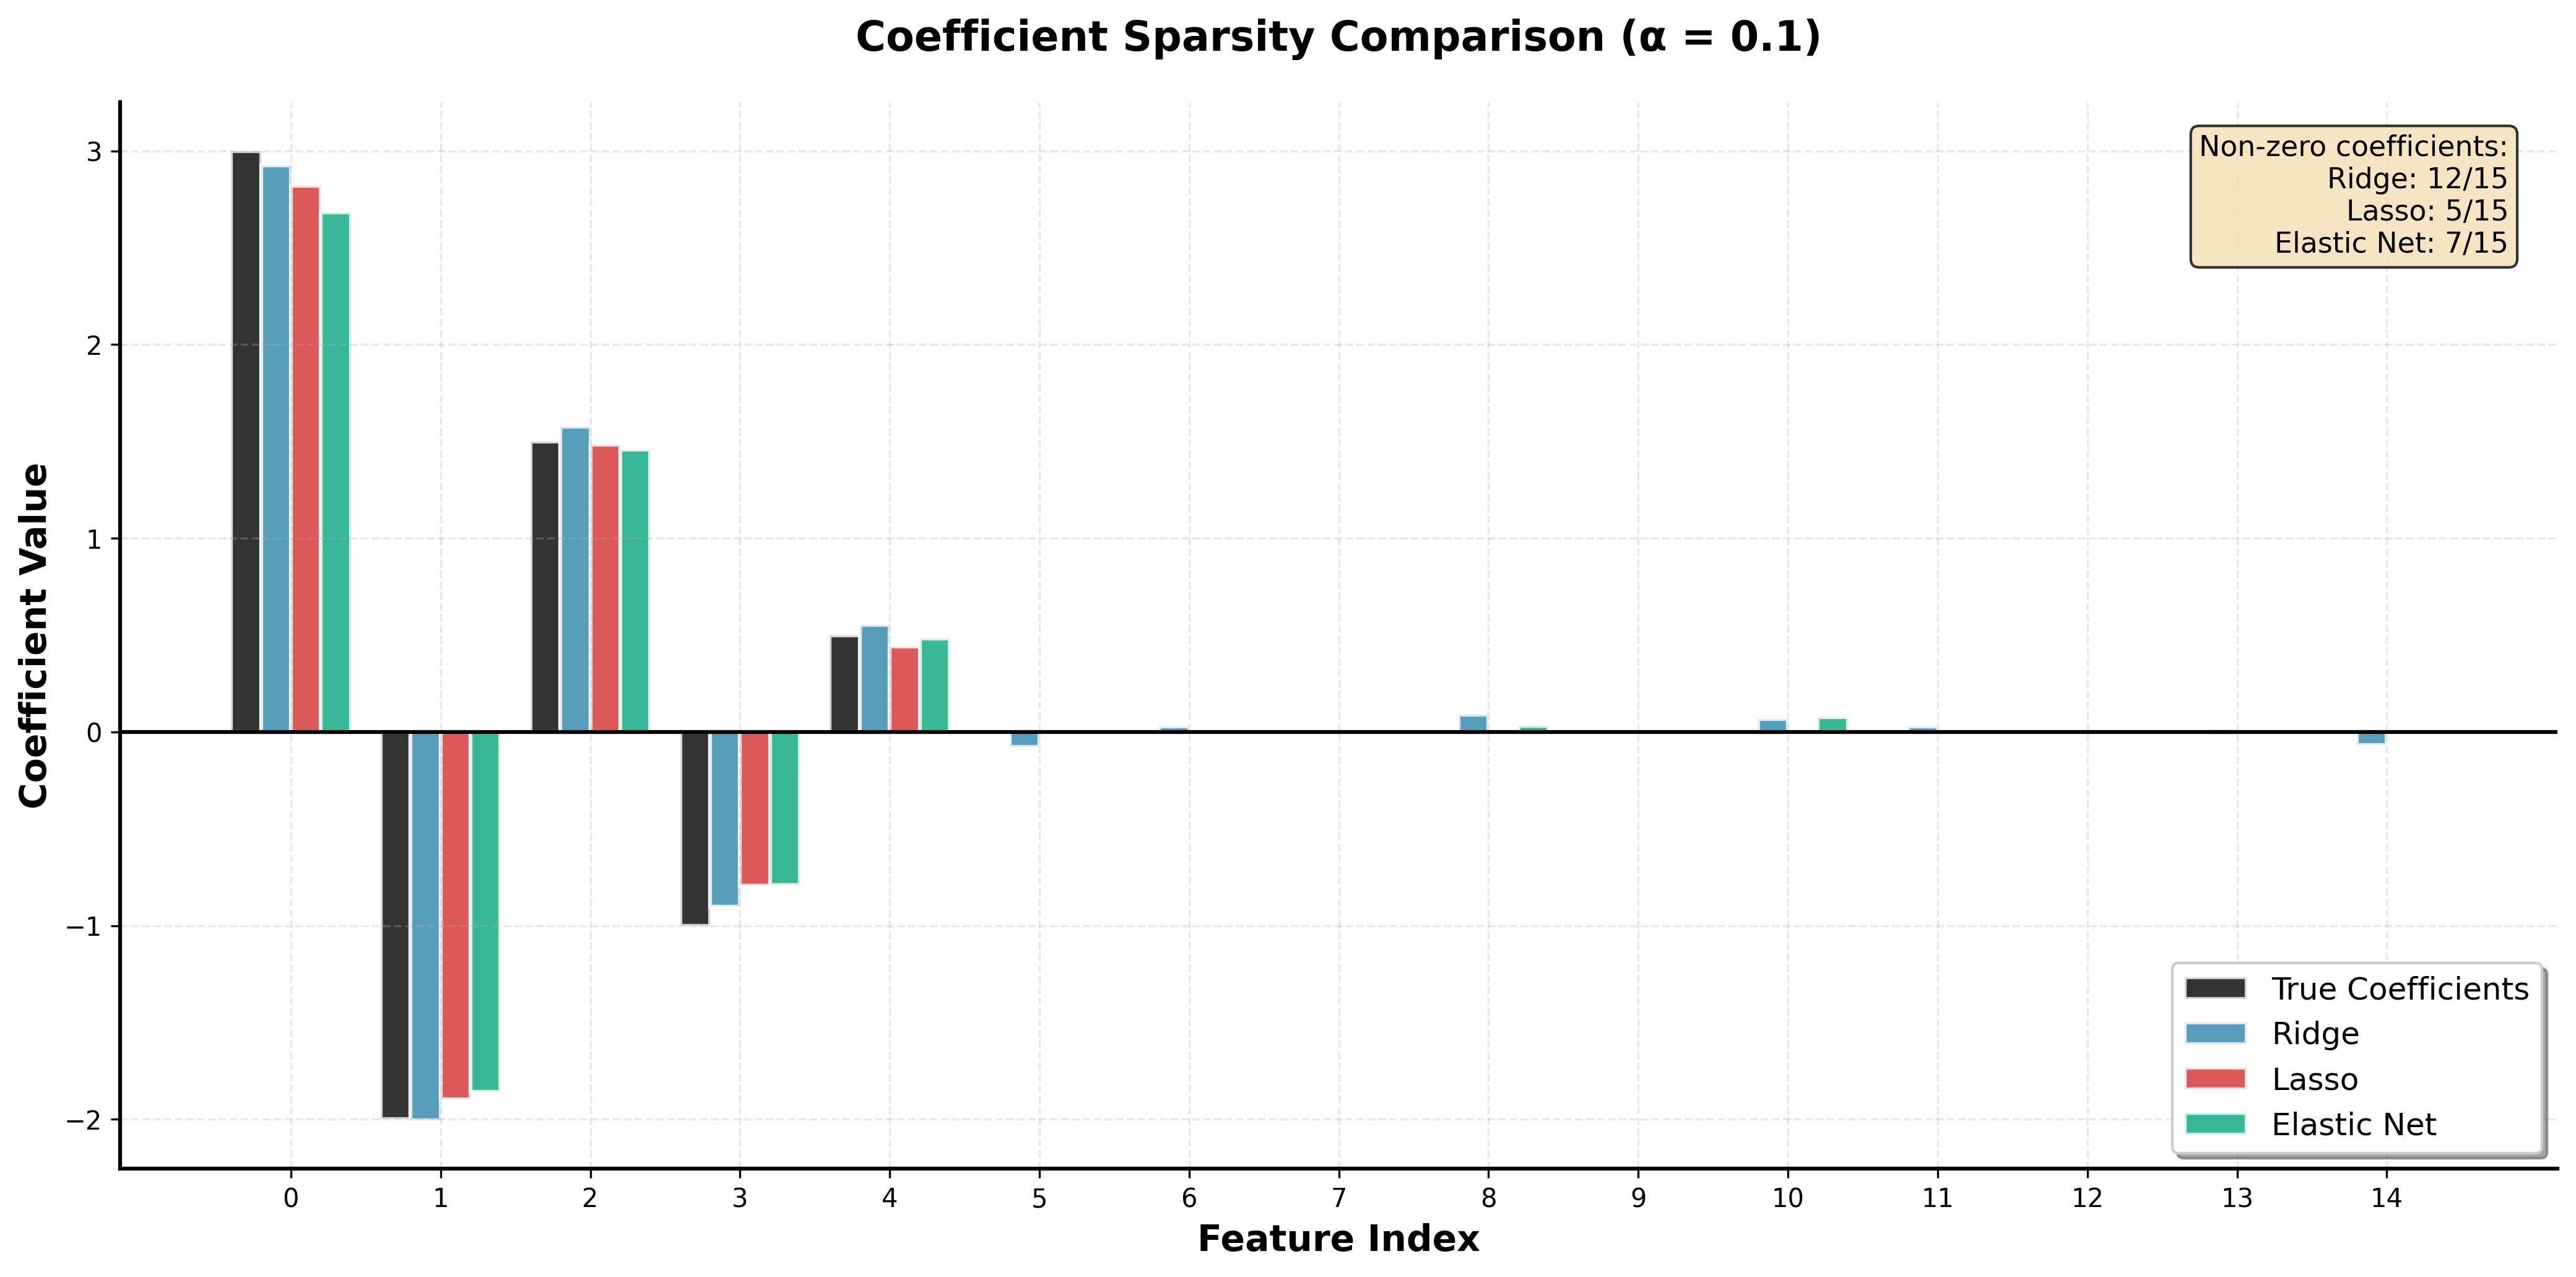
\includegraphics[width=\textwidth]{../figures/sparsity_comparison.png}
\end{center}
\end{column}
\end{columns}
\end{frame}

\begin{frame}{L1 vs L2 Regularization: Geometric Interpretation}
\begin{center}
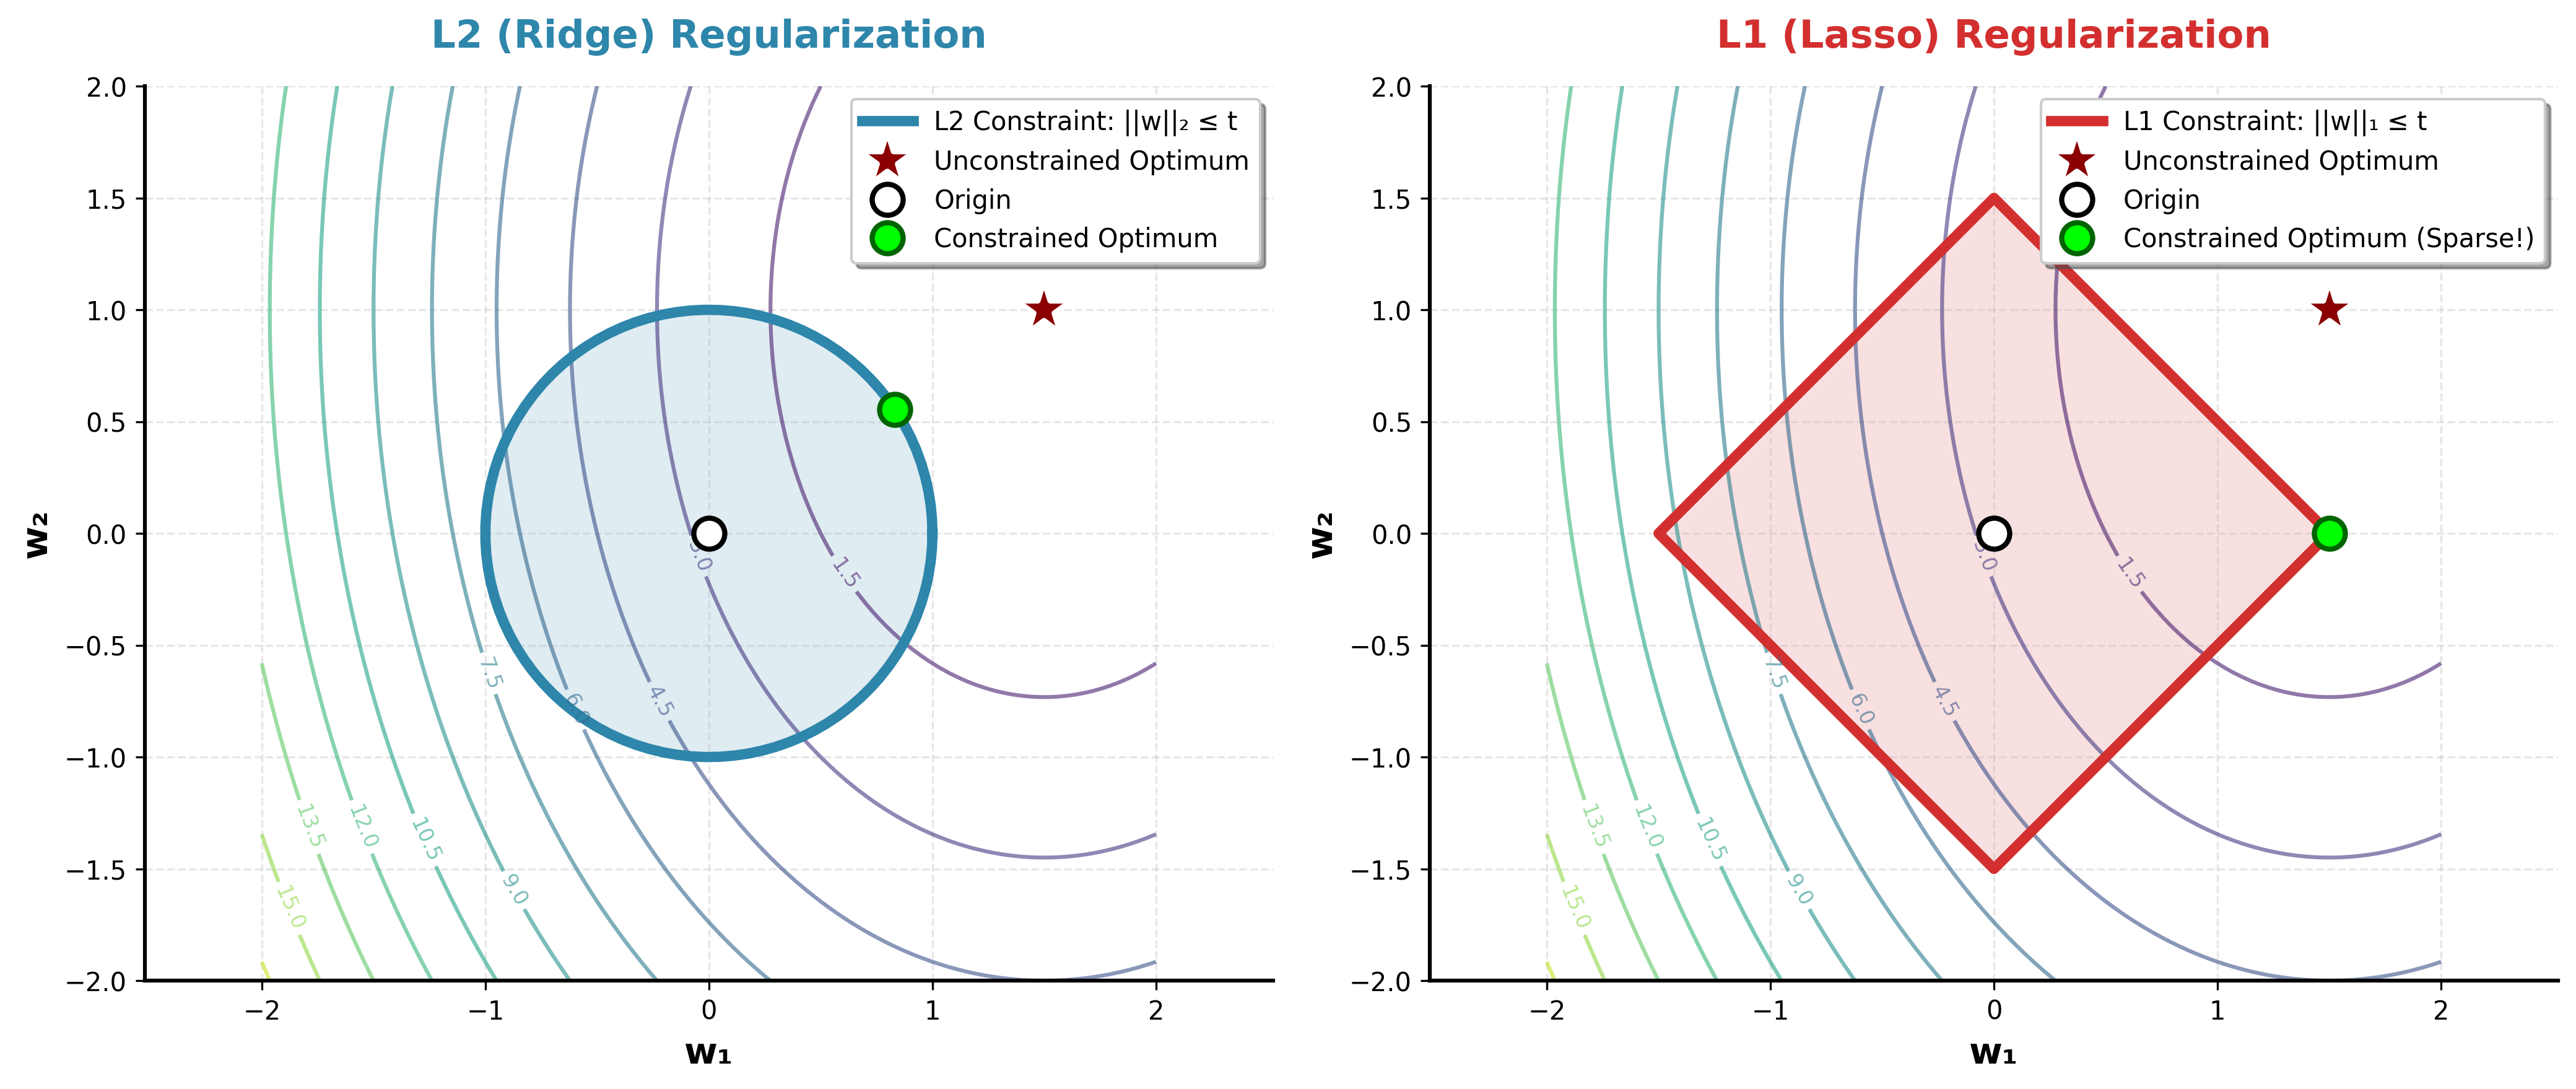
\includegraphics[width=0.85\textwidth]{../figures/l1_vs_l2_geometry.png}
\end{center}

\vspace{0.1cm}

\begin{itemize}
\item \textbf{L2 (Ridge):} Circular constraint region - solution rarely at axes (non-sparse)
\item \textbf{L1 (Lasso):} Diamond constraint region - corners encourage sparse solutions
\item Contours represent loss function, constraint region represents penalty
\end{itemize}
\end{frame}

\begin{frame}{Regularization Paths}
\begin{center}
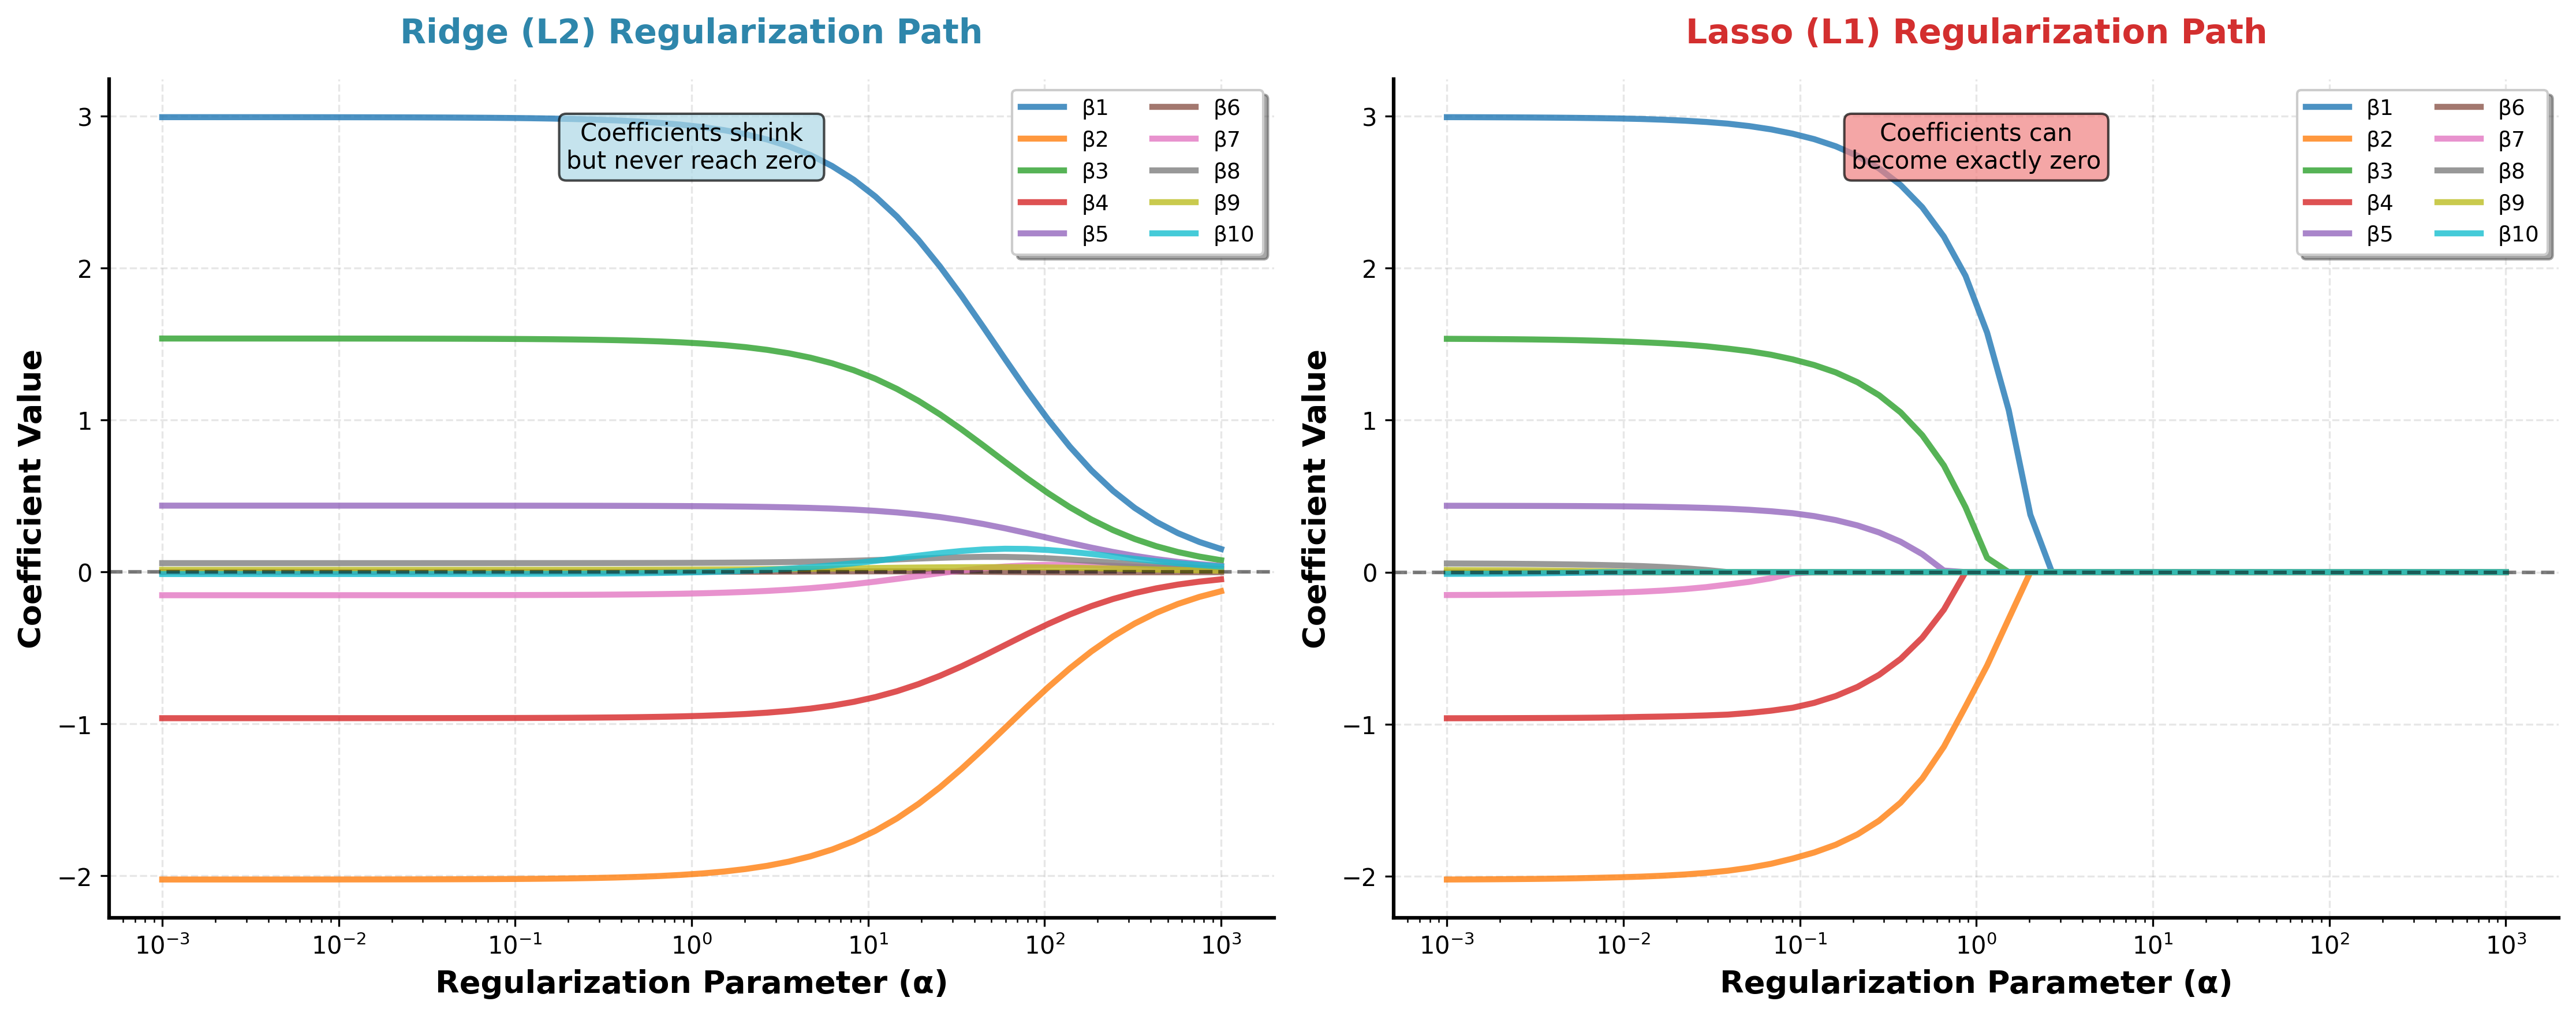
\includegraphics[width=0.85\textwidth]{../figures/regularization_paths.png}
\end{center}

\vspace{0.1cm}

\begin{techblock}{Observations}
\begin{itemize}
\setlength{\itemsep}{2pt}
\item \textbf{Ridge:} Coefficients shrink smoothly but never reach exactly zero
\item \textbf{Lasso:} Coefficients can become exactly zero at finite $\lambda$
\item As $\lambda \to \infty$, all coefficients approach zero
\item Different coefficients zero out at different $\lambda$ values in Lasso
\end{itemize}
\end{techblock}
\end{frame}

\begin{frame}{Elastic Net: Combining L1 and L2}
\begin{block}{Objective Function}
\vspace{-0.1cm}
\begin{equation*}
\min_{\mathbf{w}} \sum_{i=1}^{n}(y_i - \mathbf{w}^T\mathbf{x}_i)^2 + \lambda_1 \|\mathbf{w}\|_1 + \lambda_2 \|\mathbf{w}\|_2^2
\end{equation*}
Alternatively parameterized with mixing parameter $\alpha \in [0,1]$:
\begin{equation*}
\text{Penalty} = \lambda \left[ \alpha \|\mathbf{w}\|_1 + (1-\alpha) \|\mathbf{w}\|_2^2 \right]
\end{equation*}
\end{block}

\vspace{0.2cm}

\begin{columns}[t]
\begin{column}{0.48\textwidth}
\begin{exampleblock}{Advantages}
\begin{itemize}
\setlength{\itemsep}{2pt}
\item Combines benefits of Ridge and Lasso
\item Handles correlated features better than Lasso
\item Can select groups of correlated features
\item More stable than Lasso
\end{itemize}
\end{exampleblock}
\end{column}

\begin{column}{0.48\textwidth}
\begin{tipblock}{When to Use}
\begin{itemize}
\setlength{\itemsep}{2pt}
\item Many correlated features
\item Want feature selection and grouping
\item Lasso is too aggressive
\item Ridge is not sparse enough
\end{itemize}
\end{tipblock}
\end{column}
\end{columns}
\end{frame}

\begin{frame}{Comparing Regularization Methods}
\begin{center}
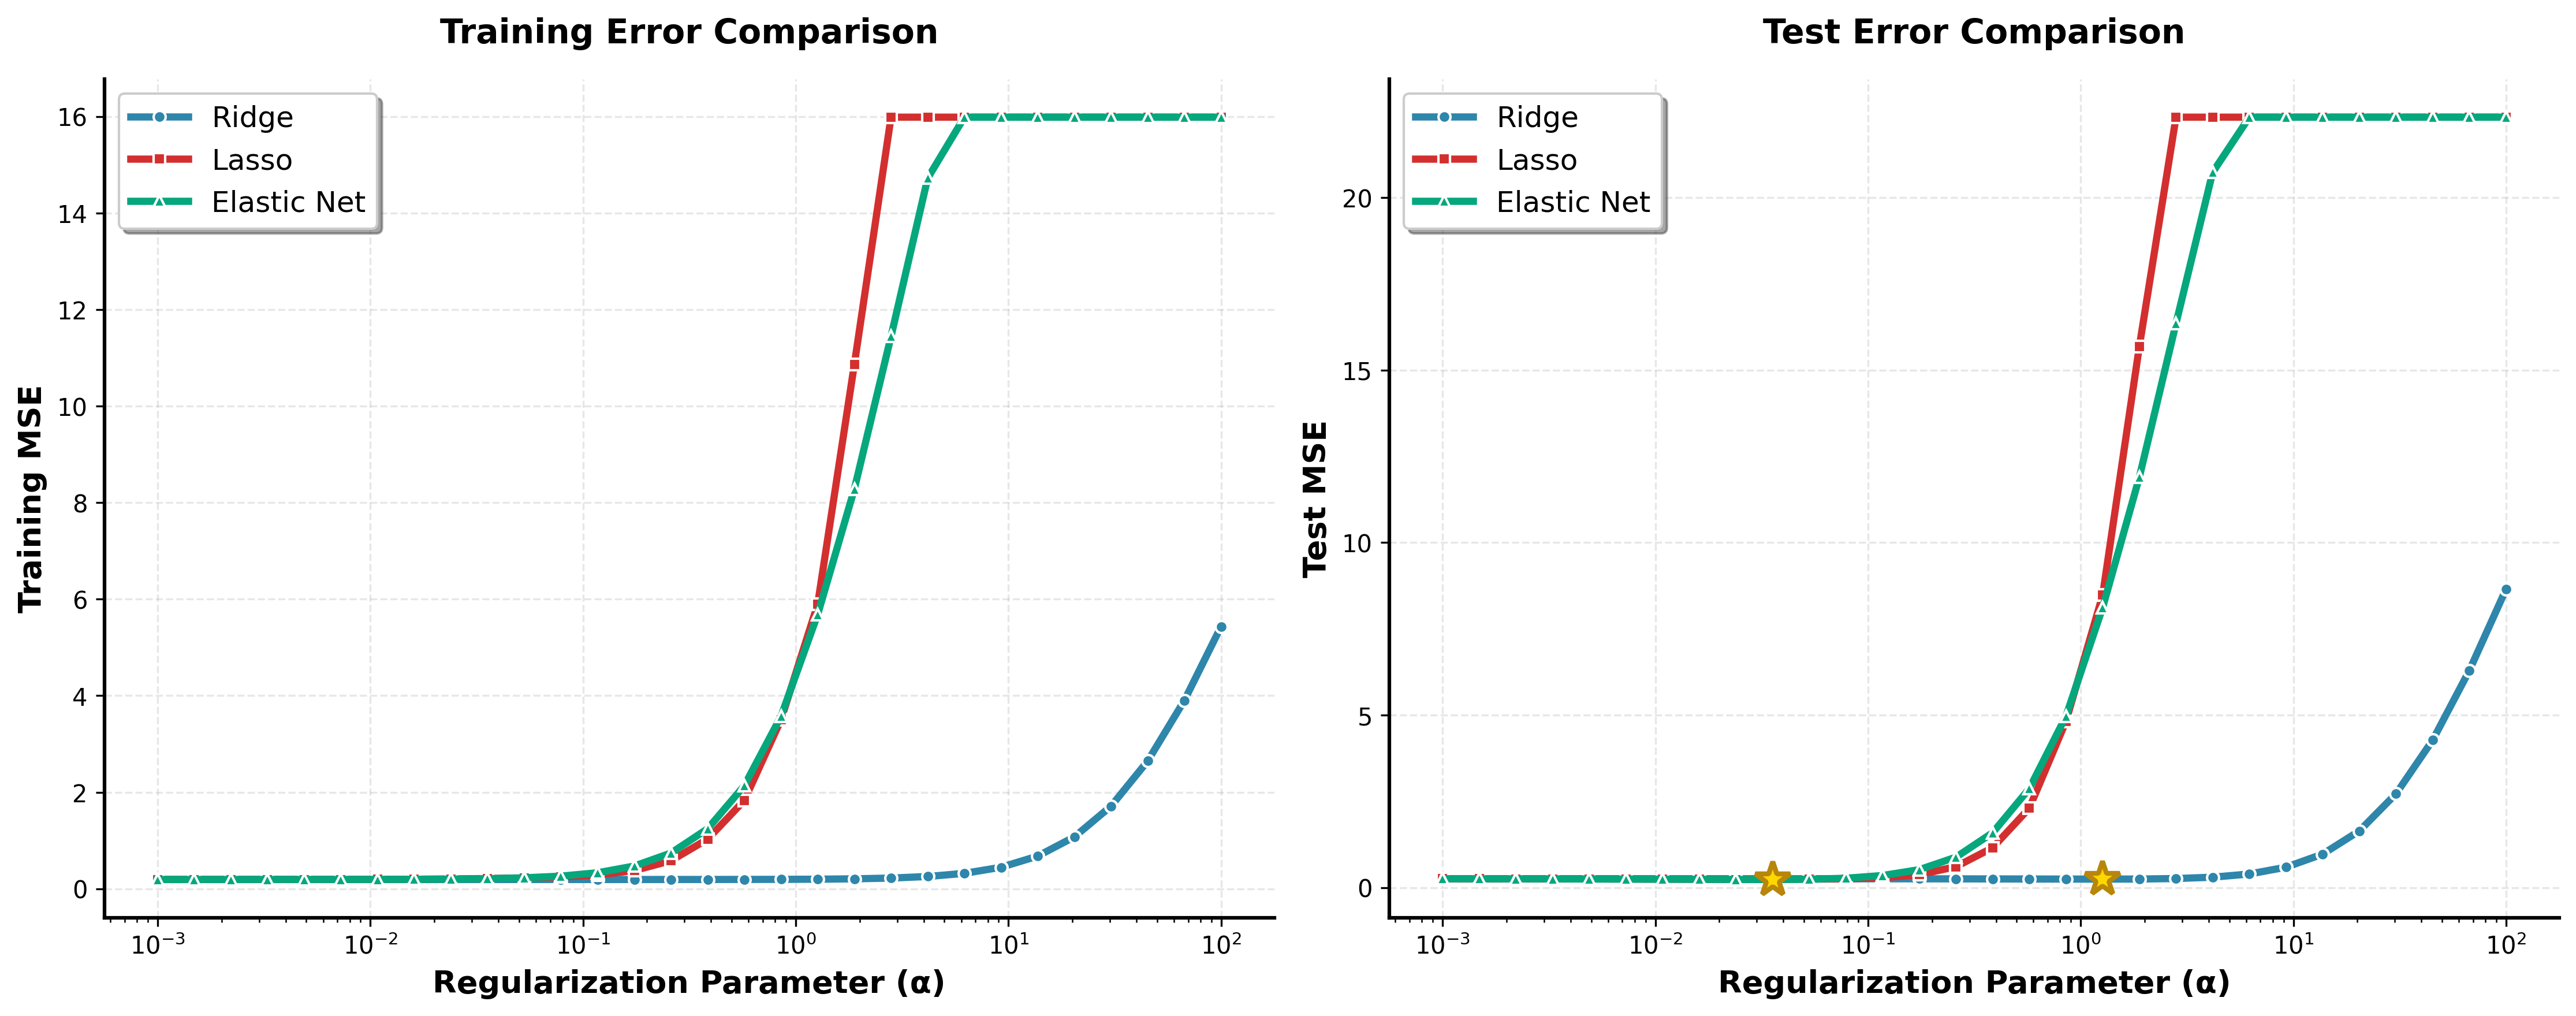
\includegraphics[width=0.85\textwidth]{../figures/regularization_comparison.png}
\end{center}

\vspace{0.1cm}

\begin{itemize}
\item All methods converge to similar training error with strong regularization
\item Test error differences reveal generalization capabilities
\item Optimal $\lambda$ differs across methods
\end{itemize}
\end{frame}

\begin{frame}{Regularization in Other Models}
\begin{columns}[t]
\begin{column}{0.48\textwidth}
\begin{block}{Neural Networks}
\begin{itemize}
\setlength{\itemsep}{2pt}
\item \textbf{Weight decay:} L2 penalty on weights
\item \textbf{Dropout:} Randomly drop neurons during training
\item \textbf{Early stopping:} Stop training before overfitting
\item \textbf{Batch normalization:} Normalize activations
\end{itemize}
\end{block}

\vspace{0.1cm}

\begin{block}{Support Vector Machines}
\begin{itemize}
\setlength{\itemsep}{2pt}
\item $C$ parameter controls regularization
\item Small $C$ = strong regularization
\item Large $C$ = weak regularization
\end{itemize}
\end{block}
\end{column}

\begin{column}{0.48\textwidth}
\begin{block}{Decision Trees/Forests}
\begin{itemize}
\setlength{\itemsep}{2pt}
\item Max depth
\item Min samples per leaf
\item Max number of features
\item Pruning
\end{itemize}
\end{block}

\vspace{0.1cm}

\begin{block}{General Strategies}
\begin{itemize}
\setlength{\itemsep}{2pt}
\item Data augmentation
\item Feature selection
\item Ensemble methods
\item Cross-validation for tuning
\end{itemize}
\end{block}
\end{column}
\end{columns}
\end{frame}

% ========================================
% Section: Best Practices
% ========================================

\section{Best Practices and Common Pitfalls}

\begin{frame}{Model Selection Best Practices}
\begin{exampleblock}{Do's}
\begin{itemize}
\setlength{\itemsep}{2pt}
\item Always use separate train/validation/test sets
\item Use cross-validation for robust estimates
\item Tune hyperparameters only on validation data
\item Report final performance on test set (once!)
\item Standardize/normalize features appropriately
\item Use stratified splits for classification
\item Track both training and validation metrics
\item Document all preprocessing steps
\end{itemize}
\end{exampleblock}
\end{frame}

\begin{frame}{Common Pitfalls to Avoid}
\begin{alertblock}{Don'ts}
\begin{itemize}
\setlength{\itemsep}{2pt}
\item \textbf{Data leakage:} Including test data in preprocessing
\item \textbf{Peeking at test set:} Multiple evaluations on test set
\item \textbf{Ignoring class imbalance:} Using accuracy on imbalanced data
\item \textbf{Not checking assumptions:} Assuming i.i.d. data
\item \textbf{Overfitting validation set:} Excessive hyperparameter tuning
\item \textbf{Cherry-picking results:} Reporting only best-case performance
\item \textbf{Inadequate splitting:} Too small validation/test sets
\item \textbf{Comparing on training data:} Always compare on validation
\end{itemize}
\end{alertblock}
\end{frame}

\begin{frame}{Data Leakage: A Critical Issue}
\begin{alertblock}{What is Data Leakage?}
Information from the test/validation set leaking into the training process, leading to overly optimistic performance estimates.
\end{alertblock}

\vspace{0.2cm}

\begin{columns}[t]
\begin{column}{0.48\textwidth}
\begin{exampleblock}{Common Sources}
\begin{itemize}
\setlength{\itemsep}{2pt}
\item Normalization using all data
\item Feature selection on all data
\item Imputation using all data
\item Temporal data ordering issues
\item Duplicate samples across splits
\end{itemize}
\end{exampleblock}
\end{column}

\begin{column}{0.48\textwidth}
\begin{tipblock}{Prevention}
\begin{itemize}
\setlength{\itemsep}{2pt}
\item Split data FIRST
\item Fit preprocessing only on training
\item Transform validation/test separately
\item Use pipelines
\item Be careful with time series
\end{itemize}
\end{tipblock}
\end{column}
\end{columns}

\vspace{0.2cm}

\begin{techblock}{Example: Correct Order}
1. Split data $\to$ 2. Fit scaler on train $\to$ 3. Transform train/val/test $\to$ 4. Train model
\end{techblock}
\end{frame}

\begin{frame}{Hyperparameter Tuning Strategies}
\begin{columns}[t]
\begin{column}{0.48\textwidth}
\begin{block}{Grid Search}
\begin{itemize}
\setlength{\itemsep}{2pt}
\item Exhaustive search over grid
\item Guarantees finding best in grid
\item Exponential in \# parameters
\item Good for few parameters
\end{itemize}
\end{block}

\vspace{0.1cm}

\begin{block}{Random Search}
\begin{itemize}
\setlength{\itemsep}{2pt}
\item Randomly sample combinations
\item Often finds good solutions faster
\item Better for many parameters
\item Can set computational budget
\end{itemize}
\end{block}
\end{column}

\begin{column}{0.48\textwidth}
\begin{block}{Bayesian Optimization}
\begin{itemize}
\setlength{\itemsep}{2pt}
\item Models objective function
\item Guides search intelligently
\item Most sample-efficient
\item Good for expensive models
\end{itemize}
\end{block}

\vspace{0.1cm}

\begin{tipblock}{Practical Tips}
\begin{itemize}
\setlength{\itemsep}{2pt}
\item Start with coarse grid
\item Refine around best values
\item Use log scale for $\lambda$
\item Parallelize when possible
\end{itemize}
\end{tipblock}
\end{column}
\end{columns}
\end{frame}

\begin{frame}{Nested Cross-Validation}
\begin{columns}[t]
\begin{column}{0.55\textwidth}
\begin{alertblock}{Problem}
Using CV for both model selection and performance estimation gives biased results!
\end{alertblock}

\vspace{0.1cm}

\begin{exampleblock}{Solution: Nested CV}
\begin{itemize}
\setlength{\itemsep}{2pt}
\item \textbf{Outer loop:} Estimates true performance
\item \textbf{Inner loop:} Selects hyperparameters
\item Provides unbiased performance estimate
\item More computationally expensive
\end{itemize}
\end{exampleblock}

\vspace{0.1cm}

\begin{techblock}{Structure}
For each outer fold:
\begin{enumerate}
\setlength{\itemsep}{1pt}
\item Set aside test fold
\item Use inner CV to select hyperparameters
\item Train final model with best hyperparameters
\item Evaluate on test fold
\end{enumerate}
Average outer fold results
\end{techblock}
\end{column}

\begin{column}{0.42\textwidth}
\begin{center}
\begin{tikzpicture}[scale=0.7]
% Outer loop
\draw[thick, blue] (0,0) rectangle (5,0.6);
\node at (2.5, 0.3) {\small Outer Fold 1};

\draw[thick, blue] (0,-1) rectangle (5,-0.4);
\node at (2.5, -0.7) {\small Outer Fold 2};

\draw[thick, blue] (0,-2) rectangle (5,-1.4);
\node at (2.5, -1.7) {\small Outer Fold 3};

% Inner loops for first outer fold
\draw[thick, red] (0.2, 1.2) rectangle (1.5, 1.6);
\node at (0.85, 1.4) {\tiny Inner 1};

\draw[thick, red] (1.7, 1.2) rectangle (3, 1.6);
\node at (2.35, 1.4) {\tiny Inner 2};

\draw[thick, red] (3.2, 1.2) rectangle (4.5, 1.6);
\node at (3.85, 1.4) {\tiny Inner 3};

% Arrows
\draw[->, thick] (2.5, 0.6) -- (2.5, 1.2);

% Labels
\node[blue, left] at (-0.2, 0.3) {\small Outer};
\node[red, right] at (5.2, 1.4) {\small Inner};
\end{tikzpicture}
\end{center}
\end{column}
\end{columns}
\end{frame}

\begin{frame}{Model Selection Checklist}
\begin{columns}[t]
\begin{column}{0.48\textwidth}
\begin{block}{Before Training}
\begin{itemize}
\setlength{\itemsep}{2pt}
\item[$\square$] Understand the problem and data
\item[$\square$] Check for class imbalance
\item[$\square$] Handle missing values
\item[$\square$] Split data properly
\item[$\square$] Standardize/normalize features
\item[$\square$] Choose appropriate metrics
\end{itemize}
\end{block}

\vspace{0.1cm}

\begin{block}{During Training}
\begin{itemize}
\setlength{\itemsep}{2pt}
\item[$\square$] Use cross-validation
\item[$\square$] Track train and validation metrics
\item[$\square$] Try multiple model types
\item[$\square$] Tune hyperparameters systematically
\item[$\square$] Check for overfitting
\end{itemize}
\end{block}
\end{column}

\begin{column}{0.48\textwidth}
\begin{block}{After Training}
\begin{itemize}
\setlength{\itemsep}{2pt}
\item[$\square$] Evaluate on test set (once!)
\item[$\square$] Compare multiple metrics
\item[$\square$] Analyze errors/confusion matrix
\item[$\square$] Check for biases
\item[$\square$] Document results
\item[$\square$] Assess computational requirements
\end{itemize}
\end{block}

\vspace{0.1cm}

\begin{alertblock}{Golden Rule}
\textbf{Never} touch the test set until final evaluation, and evaluate on it only \textbf{once}!
\end{alertblock}
\end{column}
\end{columns}
\end{frame}

% ========================================
% Section: Summary
% ========================================

\section{Summary and Key Takeaways}

\begin{frame}{Summary: Key Concepts}
\begin{enumerate}
\item \textbf{Bias-Variance Tradeoff}
\begin{itemize}
\item Balance between model complexity and generalization
\item Underfitting (high bias) vs Overfitting (high variance)
\end{itemize}

\vspace{0.1cm}

\item \textbf{Model Validation}
\begin{itemize}
\item Always use separate train/validation/test sets
\item Cross-validation provides robust performance estimates
\item Learning curves diagnose fitting issues
\end{itemize}

\vspace{0.1cm}

\item \textbf{Evaluation Metrics}
\begin{itemize}
\item Choose metrics appropriate for the problem
\item Classification: accuracy, precision, recall, F1, ROC-AUC
\item Regression: MSE, RMSE, MAE, $R^2$
\end{itemize}

\vspace{0.1cm}

\item \textbf{Regularization}
\begin{itemize}
\item Ridge (L2): shrinks coefficients, keeps all features
\item Lasso (L1): feature selection via sparsity
\item Elastic Net: combines L1 and L2
\end{itemize}
\end{enumerate}
\end{frame}

\begin{frame}{Key Takeaways}
\begin{alertblock}{Critical Principles}
\begin{itemize}
\setlength{\itemsep}{3pt}
\item \textbf{Generalization is the goal} - training performance is not enough
\item \textbf{Avoid data leakage} - fit preprocessing only on training data
\item \textbf{Use proper validation} - cross-validation for robust estimates
\item \textbf{Test set is sacred} - evaluate on it only once at the end
\item \textbf{Choose appropriate metrics} - align with business/research goals
\item \textbf{Regularize when needed} - prevent overfitting proactively
\item \textbf{Document everything} - ensure reproducibility
\end{itemize}
\end{alertblock}

\vspace{0.2cm}

\begin{techblock}{Next Steps}
Practice model selection and evaluation on real datasets using cross-validation, regularization, and proper evaluation protocols.
\end{techblock}
\end{frame}

\begin{frame}{Additional Resources}
\begin{block}{Textbooks}
\begin{itemize}
\item Hastie, Tibshirani, Friedman - \textit{The Elements of Statistical Learning}
\item Bishop - \textit{Pattern Recognition and Machine Learning}
\item James et al. - \textit{An Introduction to Statistical Learning}
\end{itemize}
\end{block}

\vspace{0.2cm}

\begin{block}{Online Resources}
\begin{itemize}
\item scikit-learn documentation: Model selection and evaluation
\item Coursera: Machine Learning by Andrew Ng
\item Fast.ai: Practical Deep Learning for Coders
\end{itemize}
\end{block}

\vspace{0.2cm}

\begin{center}
\textbf{\Large Thank you!}
\end{center}
\end{frame}

\end{document}
